\section{\I{The population section}\label{sec:population-section}}

\subsection{Introduction}
The population section\index{Population section} (Section\ref{sec:population-section}) specifies the dynamics that occur to agents in a population over time. They are labelled as population level processes such as death, birth, migration and growth but all occur at an agent level. For each process we will define the algorithm and mathematical representation and an example of the syntax for how you would incorporate in your own model. This section also discusses how to define the temporal and spatial resolution, which are completely user defined albeit some are computationally limited.

The population section consists of several components, including:
\begin{itemize}
  \item The spatial structure (Section~\ref{sec:spatial-structure});
  \item The population structure;
  \item Model initialisation (i.e., the state of the partition at the start of the first year)\index{Initialisation}\index{Model ! initialisation};
  \item The years over which the model runs (i.e., the start and end years of the model)
  \item The annual cycle (time-steps and processes that are applied in each time-step)\index{Annual cycle};
  \item The specification and parameters of the population processes (i.e., processes that add, remove individuals to or from the partition, or shift numbers between ages areas);
  \item Selectivities;
  \item Layers (used by processes, observations and reports) and their definitions
  \item Parameter values and their definitions; and
  \item Derived quantities, required as parameters for some processes (e.g. mature biomass to resolve any density dependent processes, such as the spawner-recruit relationship in a recruitment process).
\end{itemize}

\subsection{\I{Spatial structure}\label{sec:spatial-structure}}
The spatial structure of \IBM\ is represented by an $n_{rows} \times n_{cols}$ grid, with rows $i=1 \dots n_{rows}$ and columns $j=1 \ldots n_{cols}$. Each cell of this matrix records the population structure at that point in space, where the population structure is represented by a vector of agents. Locations where agents can and cannot potentially be present using a \emph{layer}. 

\IBM\ implements a single spatial structure, a grid of \emph{square} cells (Figure \ref{fig:SquareSpatialStructure}). The spatial grid can be of an arbitrary size, but must be rectangular. 

The dimensions of the spatial grid are user defined but must be at least a $1 \times 1$ grid (i.e., a single spatial cell), and the largest spatial structure currently allowed by \IBM\ is a grid of $1000 \times 1000$ cells\index{Maximum size of the spatial grid} -- although we note that models of this size are untested and will probably have very long run times. 

Associated with the $n_{rows} \times n_{cols}$ spatial structure is the one compulsory layer (see Section \ref{sec:layers}), the \emph{base layer}\index{Base layer}. This defines the locations where agents can and cannot be present (e.g., in a marine model, the locations associated with the sea and not land). These are defined as the cells where the base layer has a value greater than zero. There must be at least one cell in the spatial grid where the population can be present. In addition, the base layer also defines the relative \emph{area}\index{Cell area} of each spatial cell that is used for density calculations within \IBM.

\begin{figure}[htp]
	\centering
	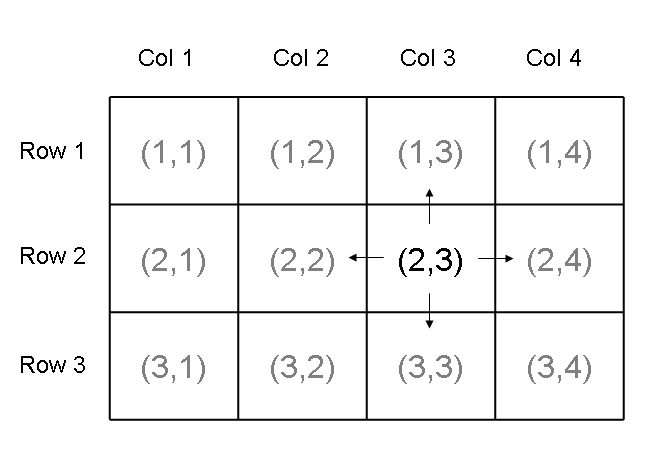
\includegraphics[width=0.66\textwidth]{Figures/SquareStructure}
	\caption{An illustration of the spatial structure}
	\label{fig:SquareSpatialStructure}
\end{figure}

Models are implemented as a grid of square cells making up a rectangular matrix.

Hence, the definition of the spatial structure includes;
\begin{itemize}
	\item The type of spatial grid and its dimensions, $n_{rows}$ and $n_{cols}$
	\item The label of a numeric layer to be used as the base layer (defining the locations where the population can be present as well as the area of each cell)
\end{itemize}

For example, to specify a model with 3 rows and 4 columns (i.e., 12 spatial cells) with a base layer called \texttt{base}, then the syntax for \texttt{@model} would include,
{\small{\begin{verbatim}
		@model
		nrows 3
		ncols 4
		layer base
		\end{verbatim}}}

See Section~\ref{sec:layers} for how to define a layer using \command{layer}. Some processes reports require the user to define latitude and longitude bounds for cells. As they are cell bounds the model expects one more bound than rows or columns. The format of latitude and longitude are 0-180 and 0-360, respectively.


\subsection{\I{Population structure}}\label{sub:sec:pop_sec}
The basic structure of the population section of a \IBM\ model is defined in terms of an annual cycle, time steps, states, and transitions.

The annual cycle defines what processes happen in each model year, and in what sequence. \IBM\ runs on an annual cycle rather than, for example, a 6-monthly cycle.

Each year is split into one or more time steps, with at least one process occurring in each time step. Each time step can be thought of as representing a particular part of the calendar year, or time steps can be treated as an abstract sequence of events. In every time step, there exists a mortality block: a group of consecutive mortality-based processes, where individuals are deleted from the population (see Section~\ref{sec:mortality_block}). This is an important concept to understand as derived quantities and some observations are associated with mortality blocks.

The division of the year into an arbitrary number of time steps allows the user to specify the exact order in which processes and observations occur throughout the year. The user needs to specify the time step in which each process occurs. If more than one process occurs in the same time step, the order in which to apply each process is specified in the \command{time\_step} block.

The state is the current status of the population which is made of a collection of agents at any given time. The state can change one or more times in each time step of every year. The state object must contain sufficient information to figure out how the underlying population changes over time (given a model and a complete set of parameters).

The state can undergo a number of possible changes, called transitions. Transitions are accomplished by processes, including: recruitment, natural mortality, anthropogenic mortality, movement, tagging events, growth, and maturation. 

The key element of the state is the spatial world view, which holds all the entities, and is described earlier in Section~\ref{sec:spatial-structure}.

An example of syntax, to specify a model with the the above concepts is done using the \texttt{@model} block is specified as:
{\small{\begin{verbatim}
		@model
		start_year 1970
		final_year 2018
		min_age 1
		max_age 20
		nrows 2
		ncols 4
		age_plus_group True
		initialisation_phases iterative
		time_steps Summer Autumn Winter Spring
		
		@time_step Summer
		processes recruitment summer_fishery 

		@time_step Autumn
		processes migrate_off_shore
		...
\end{verbatim}}}


\subsection{\I{Agents}\label{sec:individuals}}
An agent is the core object in the state that everything manipulates or summarises. An individual has a list of predefined attributes that the user can choose to incorporate in the model or ignore, the list is below.

\begin{itemize}
	\item age
	\item length
	\item weight
	\item sex
	\item maturity
	\item current area, birth area
	\item lat and long
	\item \I{population scalar} how many individuals does this agent represent = 1 means an individual based model (scalar)
	\item natural mortality parameter
	\item growth parameters
	\item scalar (if > 1 then this individual represents more than one is a stock specific attribute)
\end{itemize}

An important attribute, if the model contains super individuals (agents) where a single agent represents many individuals with the same characteristics is the scalar parameter. This parameter is associated with a recruitment event as we use the scalers to scale up a $SSB$ to $B_0$ for a given recruitment event. This makes the scalar more of a meta-population parameter or a stock parameter in fisheries. The way a scalar is applied is through the subcommand \subcommand{recruitment\_layer\_label} where you link a cell to a recruitment process (for more information see Section~\ref{subsec:initialisation}). This link says that any individual that was created by that recruitment dynamic gets a stock or recruitment scalar from that cell.

Maturity is an attribute that is activated by the maturity process (see Section~\ref{subsubsec:maturity}), it is tied to some specific derived quantities such as the type \subcommand{mature\_biomass}. You could also calculate the mature biomass on the fly, using the other derived quantities and selectivities, an example of this is shown in the maturity process section.

Sex is hard coded into the model and at this point the only way that sex effects model outcomes is through selectivities. So sex can have different maturation by age or length, and different vulnerability to mortality processes. The next additions are to have sex specific growth, which is a common occurrence in fish populations.

Lengths in the model are all defined by the length bins in on the \command{model}, it is important to note that all calculations that are made via length are via the mid points of the bins supplied. Users supply lower and upper bins for the length classes and all calculations are based on the mid-points.

The other attributes don't need any explanations are usually modified by processes, such as growth, movement and mortality. The attribute that I will dig into a little bit more is the scalar parameter which is calculated at the end of an initialisation phase, and assumes the initialisation phase has had a long in burn-in time to represent the correct age and length distribution.

\begin{equation}
	S_s = \frac{\sum_{s = 1}^{n_s}B0_s}{\sum_{s = 1}^{n_s}SSB_s}
\end{equation}
Where $S_s$ is the global scalar that is associated to all new individuals in the system from stock $s$, $B0_s$ is the $B_0$ parameter (user defined) for stock $s$ $SSB_s$ is the related spawning stock biomass. There are processes that do modify this, and that usually consists of processes or observations that truly involve a single entity such as tagging, when this occurs adjustments are made to this scalar.

\subsection{\I{Layers}\label{sec:layers}}
Layers are a key underlying concept in \IBM. They comprise of a grid of known values, with a value for every spatial cell in the model. Layers are used by processes, observations, and outputs commands to supply spatially explicit covariates and any categorical groupings required. 

Layers are used by \IBM\ to evaluate locations where the population may be present (via the \emph{base layer}), to provide sets of known attributes or values of each spatial location (for some processes and for preference based movements), and to group or categorise cells for use by processes and observations. Layers consist of an $n_{rows} \times n_{cols}$ matrix and can be either \emph{numeric} or \emph{categorical}. 

Every model must define at least one layer, the base layer $L_B$. A layer is defined as a $n_{rows} \times n_{cols}$ matrix of values (albeit with the exception of layers that describe distance --- these are described in detail below), where the value in each cell represents a known quantity. For example layers may represent classifications, physical attributes, or some other known or assumed quantity. Typically they are provided by the user as a matrix of values, although some layers (e.g., abundance or distance layers) can be calculated by \IBM\ during a model run. 

Within \IBM, layers are used in the following contexts:
\begin{enumerate}
	\item The base layer\index{Base layer}\index{Layers ! the base layer}: The base layer $L_B$ is a special layer (there must be exactly one base layer defined within the model) that defines the locations where the population can and cannot potentially be present (e.g., locations associated with the sea and not land in a marine model). Here, we define that a cell may potentially have part of the population present if every element $L_B(i,j) \ge 0$. Further, positive values of the base layer $L_B$ represent the \emph{area} represented by that spatial cell. Note, the values in the base layer must be numeric, but cannot be a meta-layer (\emph{see below}).
	\item \I{Covariate layers}: A model may have many covariate layers, and these are used as covariates of some population or movement process (e.g., the sea floor depth may be a covariate of some movement process). The values in layers used as covariates can be either numeric or categorical.
	\item \I{Classification layers}: A model may have many classification layers, and these are used as a classification or grouping variable for aggregating data over individual spatial cells $(i,j)$, e.g., statistical areas or management areas. Such layers are typically used to aggregate the population within cells into groups so-as to allow comparison with observations. The values in layers used as classification layers must be categorical.
\end{enumerate}

\IBM\ defines the following types of layer;

\begin{enumerate}
	\item{\I{Numeric layers}\label{numeric-layer}}: A model may have many numeric layers, and these can be used as covariates of a population or movement process (e.g., depth may be a covariate of some movement process), and/or locations of event mortality. Numeric layers can contain only continuous (numeric) variables. Values for a numeric layer must be supplied for each cell by the user. Numeric layers can be rescaled to sum to some user-defined value, and unlike other layers, the values for each cell can be estimated. 
	
	For example, to specify a numeric layer for a spatial model with $3 \times 4$ cells called, say \texttt{base}, with the top left and bottom right cells set to zero and all other cells set to one and not rescaled, use,
	{\small{\begin{verbatim}
			@layer base
			type numeric
			data 0 1 1 1
			data 1 1 1 1
			data 1 1 1 0
			\end{verbatim}}}
	
	\item {\I{Categorical layers}\label{categorical-layer}}: A model may have many categorical layers, and these can be used as a classification or grouping variable for aggregating data over individual cells, e.g., management areas; or as covariates of a population or movement process. Such layers are typically used to aggregate the population within cells into groups for comparing with observations, or to apply specific movement characteristics. The values in layers used as categorical layers can contain any characters (except white space), and are interpreted as categorical values. Values for a categorical layer must be supplied for each cell by the user.
	
	For example, to specify a categorical layer for a spatial model with $3 \times 4$ cells called, say \texttt{zone}, with the top left cells allocated as zone \texttt{A}, the bottom right allocated as zone \texttt{C}, and the rest as zone \texttt{B}, then use,
	{\small{\begin{verbatim}
			@layer zone
			type categorical
			data A A B B
			data A A C C
			data B B C C
			\end{verbatim}}}
	
	
	\item{\I{Abundance layers}}: The abundance layer is the sum of the number of individuals within cell $a$ in categories $k$ and with selectivity $S_l$ at age $l$. 
	\begin{equation}
	N(a) = \sum\limits_{k} \sum\limits_l S_l \ \text{element}(i,j,k,l)
	\end{equation}
	\IBM\ calculates the values of the layer when running the model at the point in time where the value is required.
	
	For example, to specify an abundance layer of all individuals who are categorised as \texttt{mature}, use,
	{\small{\begin{verbatim}
			@layer Abundance
			type abundance
			categories mature
			selectivities One
			\end{verbatim}}}
	
	\item {\I{Biomass layers}}: The biomass layer is the sum of the biomass of individuals within cell $a$ in categories $k$, with selectivity $S_l$ at age $l$, and mean weight $w_{kl}$
	\begin{equation}
	N(a) = \sum\limits_{k} \sum\limits_l w_{k,l} S_l \ \text{element}(i,j,k,l) 
	\end{equation}
	\IBM\ calculates the values of the layer when running the model at the point in time where the value is required.
	
	For example, to specify a biomass layer of all individuals who are categorised as \texttt{mature}, use,
	{\small{\begin{verbatim}
			@layer Biomass
			type biomass
			categories mature
			selectivities One
			\end{verbatim}}}
	
	\item {\I{Abundance-density layers}}: The abundance density layer is the density of the number of individuals within cell $a$ with area $A_a$ in categories $k$, with selectivity $S_l$ at age $l$,
	\begin{equation}
	N(a) = \frac{1}{A_a} \sum\limits_{k} \sum\limits_l S_l \ \text{element}(i,j,k,l)
	\end{equation}
	\IBM\ calculates the values of the layer when running the model at the point in time where the value is required.
	
	For example, to specify an abundance density layer of all individuals who are categorised as \texttt{mature}, use,
	{\small{\begin{verbatim}
			@layer AbundanceDensity
			type abundance_density
			categories mature
			selectivities One
			\end{verbatim}}}
	
	\item {\I{Biomass-density layers}}: The biomass-density layer is the density of the biomass of individuals within cell $a$ with area $A_a$ in categories $k$, with selectivity $S_l$ at age $l$, and mean weight $w_{kl}$,
	\begin{equation}
	N(a) = \frac{1}{A_a} \sum\limits_{k} \sum\limits_l w_{k,l} S_l \ \text{element}(i,j,k,l)
	\end{equation}
	\IBM\ calculates the values of the layer when running the model at the point in time where the value is required.
	
	For example, to specify a biomass density layer of all individuals who are categorised as \texttt{mature}, use,
	{\small{\begin{verbatim}
			@layer BiomassDensity
			type bioomass_density
			categories mature
			selectivities One
			\end{verbatim}}}

	\item {\I{Meta-layers}\label{meta-layers}}: \IBM\ defines a special type of layer known as a \emph{meta-layer}. Meta-layers allows individual layers to be indexed by year and applied as an annually varying layer within the model. For example, assume a model that uses Sea Surface Temperature (SST) as a layer, perhaps to drive some movement process. The SST values for each year of the model would be defined as individual layers, each with a unique label. A meta-layer could be defined that indexed the individual annual SST layers by year, and used as a covariate layer in the movement process. Meta-layers have a \emph{default} layer that is used for time periods that are not specifically defined. Meta layers can be used wherever ordinary layers are used (except that they cannot be used as the base layer), with \IBM\ extracting the appropriate layer value corresponding to the year or the initialisation phase.
	
	\begin{enumerate}
		
		\item {\I{Numeric meta-layers}\label{numeric meta-layer}}: Numeric meta-layers are a meta layer of numeric layers --- the individual ordinary layers that make up the meta-layer must all be of numeric type. For example, assuming that the layers \texttt{SST} and \texttt{SST1990}, \texttt{SST1995}, etc., are defined elsewhere, then to specify a numeric meta-layer with specific values for the years 1990-1995, and a default for all other years (including the initialisation phases), use, 
		
		{\small{\begin{verbatim}
				@layer AnnualSST
				type numeric_meta
				default_layer SST
				years    1990    1991    1992    1993    1994    1995
				layers SST1990 SST1991 SST1992 SST1993 SST1994 SST1995
				\end{verbatim}}}
		
		\item {\I{Categorical meta-layers}\label{categorical meta-layer}}: Categorical meta-layers are a meta layer of categorical layers --- the individual ordinary layers that make up the meta-layer must all be of categorical type. Categorical meta-layers are specified in the same way as numeric meta-layers. For example, assuming that the layers \texttt{zones} and \texttt{zone1990}, \texttt{zone1995}, etc., are defined elsewhere, then to specify a categorical meta-layer with specific values for the years 1990-1995, and a default for all other years (including the initialisation phases), use, 
		
		{\small{\begin{verbatim}
				@layer AnnualCategoricalLayer
				type categorical_meta
				default_layer zones
				years     1990     1991     1992     1993     1994     1995
				layers zone1990 zone1991 zone1992 zone1993 zone1994 zone1995
				\end{verbatim}}}
	\end{enumerate}
\end{enumerate}



\subsection{\I{Time sequences}}

The time sequence of the model is defined in the following parts;
\begin{itemize}
  \item \I{Annual cycle}
  \item \I{Mortality blocks}
  \item \I{Initialisation}
  \item \I{Model run years}\textsl{}
\end{itemize}

\subsubsection{\I{Annual cycle}}
The annual cycle is implemented as a set of processes that occur, in a user-defined order, within each year. Time-steps are used to break the annual cycle into separate components, and allow observations to be associated with different time periods and processes. Any number of processes can occur within each time-step, in any order (although there are limitations around mortality based processes - see Section~\ref{sec:mortality_block}) and can occur multiple times within each time-step. Note that time-steps are not implemented during the initialisation phases (effectively, there is only one time-step), and that the annual cycle in the initialisation phases can, optionally, be different from that which is applied during the model years.

\subsubsection{\I{Mortality blocks}}\label{sec:mortality_block}

For every time step in an annual cycle there is an associated \emph{mortality block}. Mortality blocks are a key concept in \IBM.

Mortality blocks are used to define the `point' in the model time sequence when observations (see Section~\ref{sec:observation-section}) are evaluated, and derived quantities (see Section~\ref{sec:derived-quantities}) are calculated.

A mortality block is defined as a consecutive sequence of mortality processes within a time step. The processes that are mortality processes are all pre-defined in \IBM, and cannot be modified. These mortality processes are described in subsection~\ref{sec:mortality}. 

\IBM\ requires that each time step has exactly one mortality block. To achieve this, either all the mortality processes in a time step must be sequential (i.e., there can not be a non-mortality process between any two mortality processes within any one time step); or if no mortality processes occur in a time step then the mortality block is defined to occur at the end of the time step. 

\IBM\ will error out if more than one mortality block occurs in a single time step. The consequence of a mortality block is derived quantities and observations that wrap mortality blocks get executed before and after. This can be a costly exercise, if it is important that the model attributes accounts for some mortality then this is a cost that must be taken, but if, there will usually be a parameter that you could set to 0 or one and so \IBM\ will only calculate the quantity once (either before or after). For example the parameter in the derived quantities class \subcommand{proportion\_through\_mortality}.

\begin{figure}[H]
	\centering
	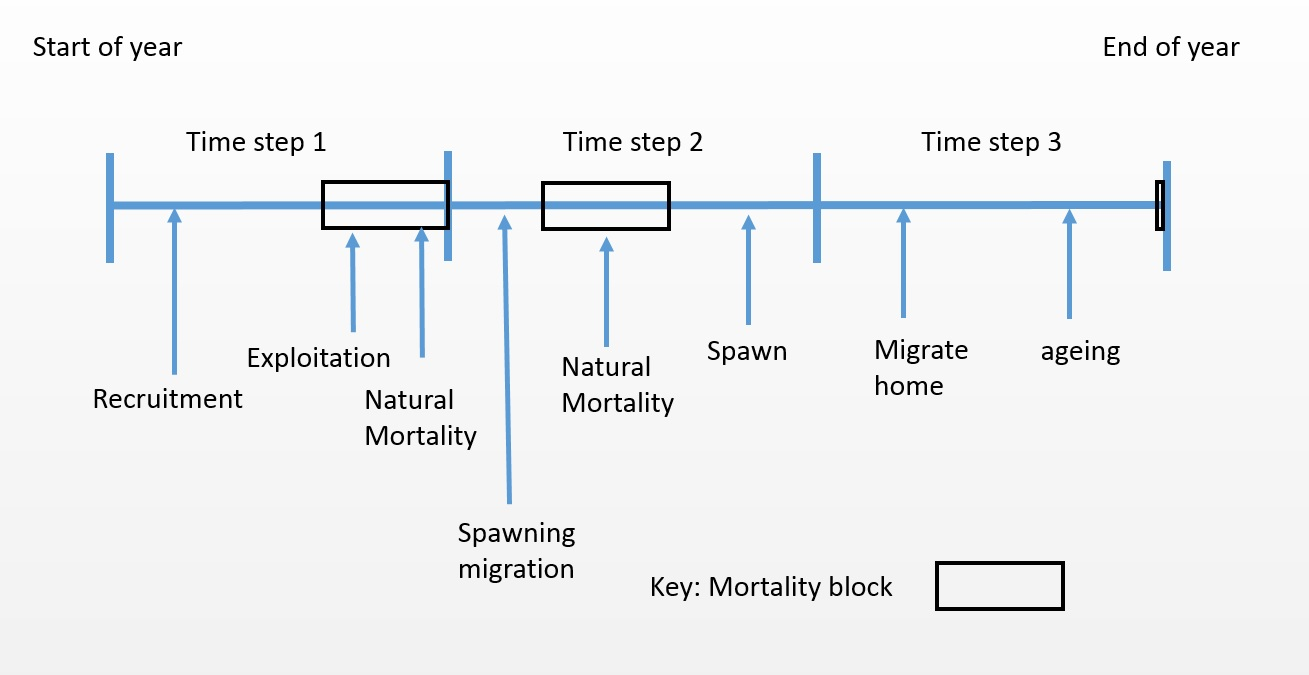
\includegraphics[scale=0.5]{Figures/annual_cycle.jpg}
	\caption{A visual representation of a hypothetical sequence for an annual cycle, with mortality blocks over multiple time steps.}\label{Fig:annual}
\end{figure}

\subsubsection{\I{Initialisation}}\label{subsec:initialisation}
Initialisation is the process of determining the world's state just before \subcommand{start\_year}, whether it be equilibrium/steady state or some other initial state for the model (e.g exploited), prior to the start year of the model. This can be computationally expensive if a plus group is present in the partition.

Currently users can only initialise the partition via an iterative method. \IBM\ does a few tricks to help speed up the initialisation. The first thing \IBM\ does is gets the parameter \subcommand{number\_of\_agents} and spits that number of agents uniformly, over the spatial domain, alternatively the user could supply a layer \subcommand{layer\_label} of proportions to seed the initial spatial distribution. This layer should sum to one so that the model initially seeds \subcommand{number\_of\_agents}. When the \IBM\ seeds the initial number of agents it also randomly assigns the agents an age based on an exponential distribution where the parameter $\lambda$ of the exponential distribution is set by the command on the \command{model}, \subcommand{natural\_mortality\_process\_label}. We suggest setting this command to the assumed natural mortality of the model. To see what age structure this would look like you can quickly use \R\ to visualise. by running the following code in an \R\ terminal you could see.

\begin{lstlisting}
Z_param = 0.2;
agents_per_cell = 1000;
hist(rexp(agents_per_cell,Z_param), breaks = 30, xlab = "age", ylab = "frequency", main = "Initial age structure in each cell")
\end{lstlisting}

Once \IBM\ has seeded the agents, it iterates over the annual cycle to change an approximated initialisation state to one that is more like what would occur for your annual cycle, this is controlled by the \subcommand{years} command in the \command{initialisation} block. The number of iterations in the iterative initialisation can effect the model output, and these should be chosen to be large enough to allow the population state to fully converge see Section~\ref{sec:tips} for some tips on initialising models.

Hence, for an iterative initialisation you need to define:
\begin{itemize}
  \item The initialisation phases,
  \item The number of years in each phase
  \item the number of individuals that you want to represent the population
  \item The initial spatial distribution of seeded agents
  \item The stock\textbackslash recruitment regions for setting the scalar.
\end{itemize}

Because the initialisation phase is responsible for seeding the initial agents, users must specify processes that the initialisation phase can seed parameters to agents. To see how parameters are set for each individual agent, users should see the individual processes in this Section~\ref{sec:process}.

An example of the syntax to implement this would be,
{\small{\begin{verbatim}
@model
...
initialisation_phases Iterative_initialisation

@initialisation_phase Iterative_initialisation
type iterative
initial_numbers_of_agents 1500000
years 50
layer_label initial_values_distribution
recruitment_layer_label recruitment_layer
\end{verbatim}}}

For an example of setting an initialisation block with multiple stocks see the 3area example.


\subsection{\I{Processes}}\label{sec:process}
Processes are a set of classes that get access to agents parameters and either modifies them (growth), moves them (to anther cell), adds new agents (recruitment) or removes them (mortality). The other thing to note is that most processes are dictated by agent specific parameters such as natural mortality and growth see specific process for more information, and usually involve a Bernoulli trial to add stochastic error. An example of this is evaluating whether an agent is caught by a fishing method, lets say that a fishing method has a length based vulnerability associated with it as shown in figure~\ref{fig:capture}


\begin{figure}[htp]\label{fig:capture}
	\centering
	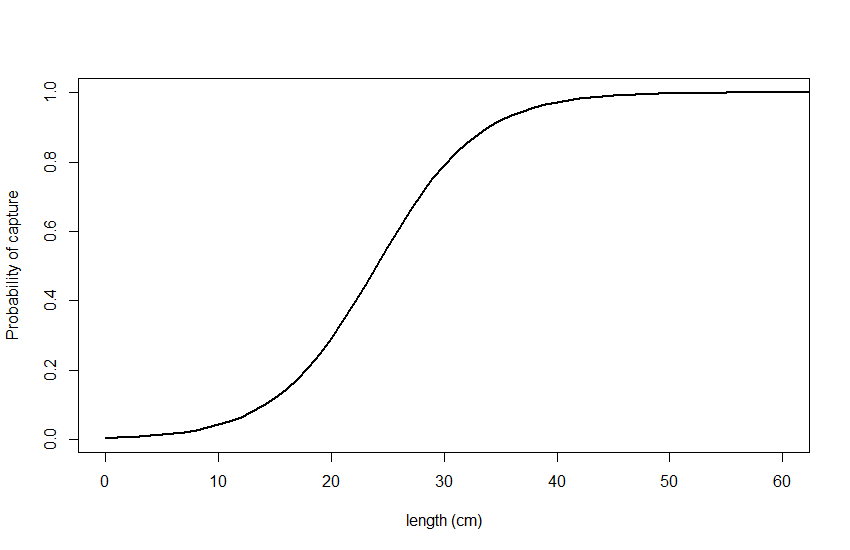
\includegraphics[scale=0.6]{Figures/vulnerability.png}%
	\caption{An example of a length based logistic vulnerability curve that describes the probability of capture when an interaction occurs.}
\end{figure}


So if we were to iterate over all the spatially available agents to this process we would calculate the probability of capture by taking the vulnerability curve and a specific agents length and compare that capture probability ($P_l$) to random number drawn from a $uniform(0,1)$ distribution denoted as$U()$, and so many of the algorithms include the term,

$$ \text{if }U() <= P_l \text{ agent is captured and removed}$$
$$ \text{else it survives the event}$$

\subsubsection{Ageing}\index{Processes!Ageing}

Ageing is an implicit process in the model, Each agent that is created or recruited gets assigned a birth year. This means that when ever we want to ask for the agent we just calculate \subcommand{current\_year - birth\_year}, thus there is no explicit ageing process. Note that we do return the \subcommand{max\_age} of the model, if the agent is older than that age (so we only work with the truncated age distribution).


This means every fish automatically ages by one at the end of the year, or you could think of ageing a fish at the very beginning of the year (tomayto, tomahto), just be aware that you don't have control over this process. Something to keep in mind is that growth is not directly tied with ageing, that is a individual that ages one year does not also get a years worth of growth. This unlike most population based models that will usually have an implicit assumption of growth with ageing. Although if one puts a growth process at the beginning or end of an annual cycle this can be achieved. This is just a side note to keep in mind when trying to align this model with others you may want to test against.


\subsubsection{Maturity}\label{subsubsec:maturity}\index{Processes!Maturity}
The process of converting an agent from immature to mature, only should be used if you link it to a mature-biomass derived quantity (Section~\ref{para:mature_biomass}). This process only changes the internal state of an agent i.e. no material change happens to the agent. This could be useful down the track if we have dynamics that only occur to mature agents and so this internal flag can be checked against for use in a different algorithm. Maturity is applied using the ogive defined in the subcommand \subcommand{maturity\_ogive\_label} in the \command{model} block, and is applied for a single agent (assuming the agent is not already mature)

\begin{equation}
	\text{maturity }\begin{cases}
	 = 1, & \text{if } U() \leq P_a\\
	 = 0, & \text{if } U() > P_a\\
	\end{cases}
\end{equation}

where, $P_a$ is the probability of an immature agent at age $a$ becoming a mature agent. Currently maturity can only be an age based process, although this is not difficult to make a length based probability statement if someone in the future wanted this. A note about creating a logistic based maturity schedule, we recommend users use the selectivity \subcommand{type = logistic\_producing} (Section~\ref{sec:selectivities}) or a similar style of selectivity. The results will not be as expected if you use a normal logistic selectivity. This is because this is only applied to the non-mature agents and so the selectivity needs more thought than other situations where a selectivity is needed\\

\begin{figure}[htp]\label{fig:mature}
	\centering
	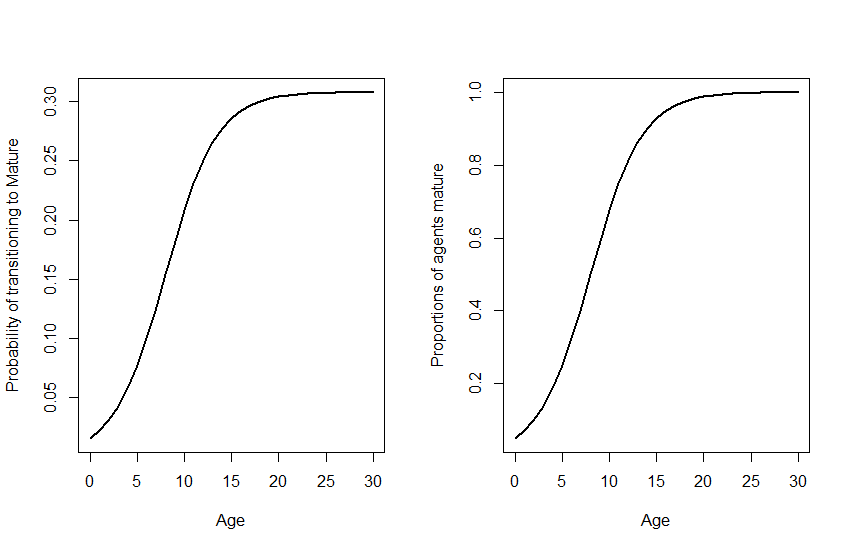
\includegraphics[scale=0.6]{Figures/maturity_ogives.png}%
	\caption{A comparison of maturity schedules, on the left we have used a logistic producing ogive, and on the right if we apply the maturity ogive over and over you get the resulting proportion mature in the right hand panel (which is logistic).}
\end{figure}


An alternative way and perhaps more efficient method for capturing a snap shot of the mature biomass or abundance of all individuals in the population is by using the generic biomass or abundance derived quantities (Section~\ref{para:biomass}~\ref{para:abundance}). Where we calculate what is mature at the time of the derived quantity, rather than having an explicit process that allows users to separate the maturation process from the summarising of abundance of biomass of the mature component. Examples of how you would set up the two methods in \IBM\ are below, firstly with maturity as an explicit process and secondly as it being implicit.

{\small{\begin{verbatim}
@model
...
maturity_ogive_label mature_ogive # define maturity selectivity: male female (order is important!!)

@time_step Annual
processes  Maturation 

@time_step Spawn
processes  no_process 

@process Maturation  # This will use the maturity ogive on the @model
type maturation

@derived_quantitiy SSB  # get a snap shot of mature biomass
type mature_biomass
time_step Spawn
biomass_layer_label SSB_areas
proportion_through_mortality_block 0.0
\end{verbatim}}}

The above model setup will have agents in the system that are mature and immature and we can call the specialised \subcommand{mature\_biomass} derived quantity to get a snap shot at any point in the system to view the biomass or abundance. The other way of dealing with maturity is implicitly as shown below.

{\small{\begin{verbatim}
@model
...
maturity_ogive_label One // define a constant selectivity here, just to keep the model happy

@time_step Annual
processes  Other_processes

@time_step Spawn
processes  no_process 	
	
@derived_quantitiy SSB  // get a snap shot of mature biomass
type biomass
time_step Spawn
selectivity mature_ogive  // Define mature selectivity here
biomass_layer_label SSB_areas
proportion_through_mortality_block 0.0
\end{verbatim}}}

So just to re-iterate the difference, you can have an explicit maturing process that is not associated with a derived quantity, or you could purely associate a derived quantity to the maturing process. This brings up a useful point in that, given the generality of the program there are more than one way to approximate dynamics and some will be more computationally quicker than others. So have a play around but try and keep the number of times we iterate over the state as small as possible, as you will get significant time saving.


\subsubsection{Recruitment}\index{Processes!Recruitment}
Recruitment is the process where new agents are created in the system. It is also the process that defines stock structure in the model. Stocks are not an explicit attribute of \IBM\ so consideration on this process is important. How the stock is defined using the recruitment dynamic surrounds where we calculate Spawning Stock Biomass ($SSB$) and where the resulting recruits are first seeded. This means that for all recruitment types you will need to specify a $B_0$ or \(R_0\) parameter and an associated derived quantity that defines the spatial resolution of the stock ($SSB$) for that event. This is how an $R_0$ value is calculated from the initialisation phase.

\begin{equation}
	X = \sum_{a = 0}^{4A}exp^{-M a}
\end{equation}

Where, $M$ is the average natural mortality rate as defined by the \subcommand{natural\_mortality\_process\_label} in the \command{model} block. $A$ is the maximum age of the population, $4$ is an arbitrary scalar to make sure that we cover the entire age distribution. Once we have our multiplier ($X$), we then


\begin{equation}
R_{0,s} = \frac{N_a}{X} \frac{B_{0,s}}{\sum_s B_{0,s}}
\end{equation}
where, $R_{0,s}$ is the stock specific initial/equilibrium number of agents to seed, $N_a$ is the number of agents in the model world defined in the \command{initialisation\_phase} using the subcommand \subcommand{number\_of\_individuals} and $B_{0,s}$ is the user defined stock specific equilibrium spawning stock biomass.

\paragraph{Constant recruitment}\label{subsubsec:constant-recruitment}\index{Processes!Recruitment!Constant recruitment}

\begin{equation}
	R_{y,s} = R_{0,s}
\end{equation}

{\small{\begin{verbatim}
# Constant
@process Recruitment_const
type recruitment_constant
recruitment_layer_label recruit_layer
b0 29924.6 
ssb SSB

@derived_quantity SSB
type mature_biomass
biomass_layer_label SSB_areas
time_step Annual
proportion_through_mortality_block 0.5

# proportion of where recruits are spatially distributed
@layer recruit_layer
type numeric
table layer
0.2 0.2 0.2
0.2 0.2 0
0 0 0
0 0 0	
end_table

# define areas where SSB calculations are made
@layer SSB_areas
type numeric
table layer
1 1 1
1 1 0
0 0 0
0 0 0	
end_table
\end{verbatim}}}
	
\paragraph{Beverton-Holt recruitment}\label{subsubsec:bev-holt-recruitment}\index{Processes!Recruitment!Beverton-Holt recruitment}

We have taken the parametrisation akin to \cite{mace_doonan_88} that is a population based formula. There is room to make this a more pure agent based model where we look at probability of finding a mate and etc, but for know this is all we have.
\begin{equation}
R_{y,s} = R_{0,s} \times \frac{SSB_{y-ssb offset,s}}{B_{0,s}}/ \left(1 - \frac{5h - 1}{4h} \left( 1 - \frac{SSB_{y-ssb offset,s}}{B_{0,s}}\right)\right) \times YCS_y
\end{equation}
where $h$ is the compensation parameter known as the steepness parameter that represents the number of agents when the stock SSB is at 20\% of $B_0$, $YCS_y$ is the year class strength parameter also termed the stock recruitment residual that accounts for any deviation of the deterministic Beverton Holt relationship due to things like predation, environment etc. If there are multiple spatial cells that are associated with a recruitment event then the allocation to a single cell is a simple multiplication with a proportion e.g.

\begin{equation}
R_{y,s,c} = R_{y,s} \times p_c
\end{equation}
where $R_{y,s,c}$ is the resulting agents in cell $c$ with proportion $p_c$ there is no stochastic behaviour in this process unlike other processes.

{\small{\begin{verbatim}
# Recruitment Beverton Holt
@process Recruitment
type recruitment_beverton_holt
recruitment_layer_label recruit_layer
b0 100000
steepness 0.85
ycs_values 1*53
ssb SSB
\end{verbatim}}}

\subsubsection{Mortality}\label{sec:mortality}\index{Processes!Mortality}
Mortality processes remove agents from the model domain, and do not allow them to be available to processes or summaries. Mortality that are associated with fishing or anthropogenic removals are also responsible for tag-recaptures.\\

Mortality types that can be used to search for tag-recaptures are, \subcommand{mortality\_event\_biomass}, \subcommand{mortality\_baranov} and \subcommand{mortality\_effort\_based}. I will describe how this is handled in \IBM\ here as the method is the same through out all three mortality processes. The inputs that will control how we sample for tag-recaptures are \subcommand{scanning\_years} and \subcommand{scanning\_proportion}. These basically just say what years we are scan for tags and what proportion of the F-mortality do we check for tags. One thing to note that has been plaguing me a little bit is the recapture probability. If you have an agent based model where an agent represents multiple individuals and you have tagging process (sub-section~\ref{subsub:tag}) which splits out a true individual. \IBM\ does not change the probability statements on how many individuals an agent represents i.e. all agents have equal probability. This means we may have the same probability of recapturing an agent that represents 10000 fish as we do an agent that represents a single individual. I haven't come up with a clever way around this, so this is purely a reminder to users to consider this before going crazy on any analysis. To extract information on tag-recaptures you will have to generate a report for the specific mortality process, as well as that you will have to specify the subcommand \subcommand{print\_extra\_info} in the \command{process} mortality block.

\paragraph{Constant mortality rate}
Apply an instantaneous mortality rate, and we remove the individual if the following condition is met which compares the survivorship ($1 - e^{-M_i * S_a}$) with a draw from a uniform random variable ($U()$).

\begin{equation}\label{constan_mort}
\text{if } U() \leq 1 - e^{-M_i * S_a} \text{ agent dies}
\end{equation}

where, $M_i$ is the individuals instantaneous mortality rate and $S_a$ is a selectivity at age allowing the process to be age based (but can be length based). $M_i$ the individuals instantaneous mortality rate is assigned from generating a random value from either a normal or lognormal distribution by using the subcommand \subcommand{distribution}

\begin{equation}\label{constan_mort_assign}
M_i \sim N(M * M_{row,col}, CV\times M * M_{row,col}) \text{ with syntax } \sim N(\mu,\sigma)
\end{equation}

or 

\begin{equation}\label{constan_mort_assign_ln}
M_i \sim LN(M * M_{row,col}, CV) \text{ with syntax } \sim LN(E[X],CV)
\end{equation}

where $M$ is the parameter \subcommand{m} and $M_{row,col}$ is the multiplier layer value in row $row$ and column $col$. For the lognormal parametrisation we make users define the expectation rather than the $\mu$ parameter as it seems more intuitive and this follows that $E[X] = e^{\mu + 0.5\sigma^2}$ Users can also set a flag (\subcommand{update\_mortality\_parameters}) that says if individuals move they will take on a new mortality rate parameter of the new area, if not they will retain their mortality rate assigned to them at birth.

An example of how you could set up a constant mortality rate process that varied through time, space and by age is below

{\small{\begin{verbatim}
@process natural_mortality
type mortality_constant_rate
update_mortality_parameters true
m_multiplier_layer_label M_layer
m 0.15
distribution lognormal
cv 0.1
selectivity_label natural_mortality_by_age

@layer M_layer
type numeric
table layer
1 1.2 1.1    # 0.15 0.18 0.165
1 0.9 0.8    # 0.15 0.135 0.12
0.8 0.8 0.7  # 0.12 0.12 0.105
end_table

@selectivity natural_mortality_by_age
type double_exponential
x1 0
x0 6
x2 30
y1 0.6
y0 0.1
y2 0.4

@time_varying m_by_year
type constant
parameter process[natural_mortality].m
values 0.134 0.153 0.106 0.1833
years 1990 1991 1992 1993 
\end{verbatim}}}

\begin{figure}[h!]
	\centering
	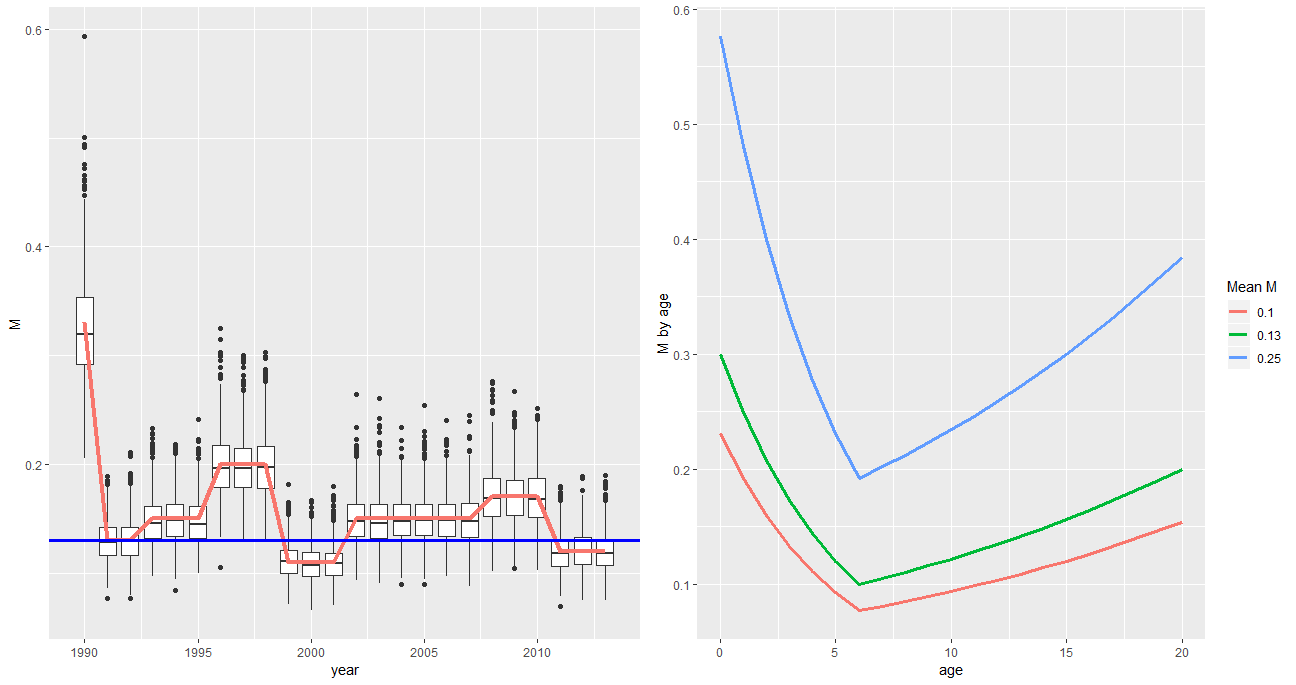
\includegraphics[scale=0.45]{Figures/Time_age_varying_M.png}
	\caption{\textbf{The left plot show how uses can vary the Mean M by year, with the blue line being the value used to initialise the agents, the red value is the input and the box and whisker's represent the actual $M$ assigned to each agent from a random sample of 1000. In the right plot we see how using selectivities the user can also have age varying $M$, here we use a double exponential curve which is demonstrated with a range of mean $M$ values that could occur in a year.}}
	\label{fig:varying_M}
\end{figure}


\paragraph{Event-Biomass}\label{para:event_mort}\index{Processes!Mortality!Event-Biomass}
This is a removal event such as fishing, where we iterate over a range of cells and remove agents based on some selectivity or spatial vulnerability. This is the simplest way to remove individuals from an anthropogenic process, however it is quite annoying to set up for a spatial model with a fine spatial resolution as you need to specify a catch for each cell. An example of how this process is set up is specified below, if you want an alternative fishing process that is based in theoretiical spatial fishing distributions see the next section (Section~\ref{para:effort_based_F}). Advantages using this mortality process say over the Baranov method (next paragraph~\ref{para:baranov}) is that it allows for agents to have multiple encounters with a fishery and it can deal with multiple fisheries with different selectivities and spatial patterns, but the negatives is that you cannot simply incorporate simultaneously natural mortality processes, and may be more suited for a pulse like fishery.\\

\textbf{The algorithm}
\begin{itemize}
	\item randomly select an agent, \textbf{with replacement}
	\item randomly select a fishery (if more than one), \textbf{with replacement}
	\item check to see if this agent is vulnerable to the fishery either age or length based process, by comparing a uniform random draw with a ogive
	\item if we are scanning fish for tag-recaptures check for tags
	\item if we have minimum legal size (MLS) check to see if the fish will be returned this is a true or false statement, if agent length $<$ MLS return with some handling mortality probability that will be again checked with a uniform random variable
	\item if not MLS check then we remove this agent from the population and add it to the catch (all agents are removed, this must be remembered)
	\item repeat the above steps until we have removed a desired biomass or if there are not enough fish to remove we exit with an error.
\end{itemize}
The key here is that an agent can interact with fishery many times during a fishing event, but there is no natural mortality.

\pagebreak
{\small{\begin{verbatim}
@process Fishing_Mortality
type mortality_event_biomass
print_extra_info true ## this may print too much information and slow down model
table catch ## these are labels for @layer that describe catch over space.
year FishingTrwl FishingLine
1972 1972_Trwl 1972_Line
1973 1973_Trwl 1973_Line
1974 1974_Trwl 1974_Line
end_table

table scanning ## proportion of catch scanned for tags
year FishingTrwl FishingLine
1972 0.3 0.5
1973 0.6 0.7
1974 0.2 0.4
end_table

## describe fishery specific parameters		
table method_info
method          male_selectivity    female_selectivity 	minimum_legel_length  handling_mortality
FishingTrwl     trwlFSel_m          trwlFSel_f			0			0
FishingLine	    Sel_Line            Sel_Line			0			0
end_table
## if single sex model only have one column called selectivity
table method_info
method        selectivity  minimum_legel_length handling_mortality
FishingTrwl   trwlFSel     0                    0
FishingLine   Sel_Line     0                    0
end_table
\end{verbatim}}}


\paragraph{ Baranov Simple}\label{para:baranov_simple}\index{Processes!Mortality!Baranov Simple}
This process applies spatially explicit fishing mortality for only a single fishery and natural mortality. See section~\ref{para:event_mort_baranov} if you want to consider multiple fisheries.

\textbf{The algorithm}
\begin{itemize}
	\item iterate over every individual in the partition or spatial cell
	\item See if the fish dies by comparing total mortality survivor ship $U() \leq 1 - e^{- M_a + F_a}$ assuming $M$ and $F$ are both age based, but they can be length based ($M_l$, $F_l$) or a combination
	\item If fish dies see if it was from $M_a$ or $F_a$ if ($U() < \frac{F_a}{F_a + M_a}$) then it was removed from an fishing event and is included in fishing specific observations.
	\item we also can apply MLS and handling survivor ship
	\item we can also choose to check for tag-recaptures
\end{itemize}
So from the algorithm above we can see that agents are exposed to both M and F, however the negative is that this assumes only a single interaction with the fishery which is an unlikely assumption. However I added this process because it both takes M and F simultaneously and may actually be faster than an event biomass dynamic (previous paragraph~\ref{para:event_mort}).


\paragraph{Baranov}\label{para:event_mort_baranov}\index{Processes!Mortality!Baranov}
This is a removal event where we iterate over a range of cells and remove agents based on multiple fisheries and spatially explicit fishing mortality rates. Advantages using this mortality process over the event biomass event (previous paragraph~\ref{para:baranov}) is that it is alot faster (computationally) another benefit is that it allows for a constant exploitation pattern, even under different recruitment trends, unlike a catch based mortality event.

for multiple fisheries, in any given cell we calculate the total fishing mortality as
\begin{align}
	F_b &= \sum_{f = 1} F_fS^f_b\\
	p^f_b &= \frac{F_fS^f_b}{F_b}
\end{align}
%,
where, \(f\) indexes the fishery, and \(S^f_b\) is the selectivity for bin \(b\) (can be either age or length) for fishery \(f\) and \(F_f\) is the fishing mortality rate in the cell we are in. \(p^f_b\) is the proportion of fishing mortality for bin \(b\) attributed ot fishery \(f\).\\
\textbf{The algorithm follows}
\begin{itemize}
	\item Iterate over each agent that is alive and see if agent \(i\) is caught ($U() < 1 - e^{F_{b_i}}$) with \(b_i\) is the bin of agent \(i\)
	\item If caught see which fishery caught it using a \(f \sim multinomial(p^f_1, \dots p^f_{n_f})\)
	\item if we have minimum legal size (MLS) check to see if the fish will be returned this is a true or false statement, if agent length $<$ MLS return with some handling mortality probability that will be again checked with a uniform random variable
	\item if not MLS check then we remove this agent from the population and add it to the catch (all agents are removed, this must be remembered)
\end{itemize}
The key here is that an agent can interact with fishery many times during the process execution, but there is no natural mortality.

\pagebreak
{\small{\begin{verbatim}
		@process Fishing_Mortality
		type mortality_baranov
		print_extra_info true ## this may print too much information and slow down table f_table
		table f_table
		 ## these are labels for @layer that describe F over space for each fishery
		year FishingTrwl FishingLine
		1972 1972_Trwl 1972_Line
		1973 1973_Trwl 1973_Line
		1974 1974_Trwl 1974_Line
		end_table
		
		## describe fishery specific parameters		
		table method_info
		method          male_selectivity    female_selectivity 	minimum_legel_length  handling_mortality
		FishingTrwl     trwlFSel_m          trwlFSel_f			0			0
		FishingLine	    Sel_Line            Sel_Line			0			0
		end_table
		## if single sex model only have one column called selectivity
		table method_info
		method        selectivity  minimum_legel_length handling_mortality
		FishingTrwl   trwlFSel     0                    0
		FishingLine   Sel_Line     0                    0
		end_table
		\end{verbatim}}}


\paragraph{Hybrid}\label{para:baranov_Hybrid}\index{Processes!Mortality!Hybrid}
\textbf{Note:} this process should only run for run mode \texttt{ibm -m}. This will apply Baranov mortality process (section~\ref{para:event_mort_baranov}) between \subcommand{start\_year} and the fisrt year in \subcommand{assessment\_years} subcomand then applies a catch based mortality \subcommand{mortality\_event\_biomass} (section~\ref{para:event_mort}) over the remaining assessment years.

The input is identical to Baranov mortality process (section~\ref{para:event_mort_baranov}) where users should only supply layer labels in table \texttt{f\_table} catch is determined by the \R\ interaction.
\paragraph{Effort-Based F}\label{para:effort_based_F}\index{Processes!Mortality!Effort-Based F}
A lot of this process was inspired by \cite{truesdell2017effects}, where users can specify some theoretical fishing distribution, currently only Ideal Free Distribution is allowed (but I am hoping to add a weighted ideal free distribution with user defined weights) and a total catch. \IBM\ applies this process by calculating the vulnerable biomass over all spatial cells ($V_{row,col}$), where each individual contributing to the vulnerable biomass is done deterministically \textbf{unlike} most other systems in the model (the stochastic nature comes later Equation~\ref{eq:catch}),

\begin{equation}
	V_{row,col} = \sum_{i\in(row,col)} \bar{w_i} \times s_i \times P_c
\end{equation}
where, $P_c$ is the probability of capture which can be length or age based, $i$ indexes all the available agents in cell $row, col$, and $\bar{w_i}$  $s_i$ are the weight and scalar of the agent respectively, $()\text{I}$ is the identity function based on the outcome of the Bernoulli trial. Once we have the vulnerable biomass by cell we want to allocate our theoretical effort. The user can specify effort two ways. The user can specify a vector of expected effort one for each enabled cell, this would mean that effort was time-invariant. The second is that user could specify a numeric layer of efforts for each year (the order is not important because \IBM\ will align them based on the theoretical distribution). \textbf{Note} units of effort could be important for solving $\lambda$ look at the end of this section to see technical details on this. Once we have effort ($E_{row,col}$) and vulnerable ($V_{row,col}$), the \IBM\ will align the highest effort value with the cell with the highest biomass, for the ideal free distribution. Once we have effort and vulnerable biomass we need to estimate a parameter $\lambda_y$ so that we solve for catch.

\begin{equation}\label{eq:catch}
\hat{C}_{y,row,col} = \sum_{i\in(row,col)} (U() \leq 1- e^{\lambda_y E_{row,col} P_c})\text{I } \bar{w_i} \times s_i
\end{equation}

A note from the above equation the uniform random draw $U()$ is set once for all agents and is not re-drawn every time we iterate over this equation to minimise the Equation~\ref{eq:minimise} below to solve for $\lambda_y$.
\begin{equation}
\hat{C}_{y} = \sum_{row}\sum_{col} \hat{C}_{y,row,col} 
\end{equation}



We then minimiser the sum of square of the following expression to solve for $\lambda_y$,

\begin{equation}\label{eq:minimise}
	\hat{\lambda}_y = argmin_{\lambda}(C_y - \hat{C}_{y})^2
\end{equation}

where, $C_y$ is the user catch, in this case $\hat{F}_y =\hat{\lambda}_y E_{row,col}$. We finally removals with our estimated $F$ using the normal survivor ship process, Bernoulli trial if $U() \leq 1- e^{\hat{F}_y P_c}$ then the agent dies.\\

A technical note to consider, is that the $\lambda$ parameter is assumed to $\lambda \in (0.0000001, 100)$. So you will need to scale and check your Effort units so that, with the above constraint and your effort we can solve for the Catch in that year. Also there is an option to specify the starting value when solving for $\lambda$ using the subcommand \subcommand{starting\_value\_for\_lambda}. If you print this process it should tell you how long it takes in seconds to solve for lambda for each year. See Section~\ref{subsec:num_diff} for information on the minimiser used in the optimisation routine.


{\small{\begin{verbatim}
@process summer_fishery
type mortality_effort_based
years 1991
catches 2234
selectivity trawl_selectivity
minimiser minimiser_for_summer_fishery
effort_values 0.076 0.089 0.219 0.104 ## for 4 cell model


@minimiser minimiser_for_summer_fishery
type numerical_differences
## play with these if you have trouble minimising or starting value
iterations	20 
evaluations 30
tolerance 0.03
step_size 0.003

\end{verbatim}}}


\paragraph{Effort-Based F with covariates}\label{para:effort_based_F_w_covars}\index{Processes!Mortality!Effort-Based F with covariates}
This process leads on from Effort-Based F above but allows for layers to control effort distribution other than vulnerable biomass. For example economic-proxy layers such as distance from the coast (Figure~\ref{fig:distance})

\begin{figure}[H]
	\centering
	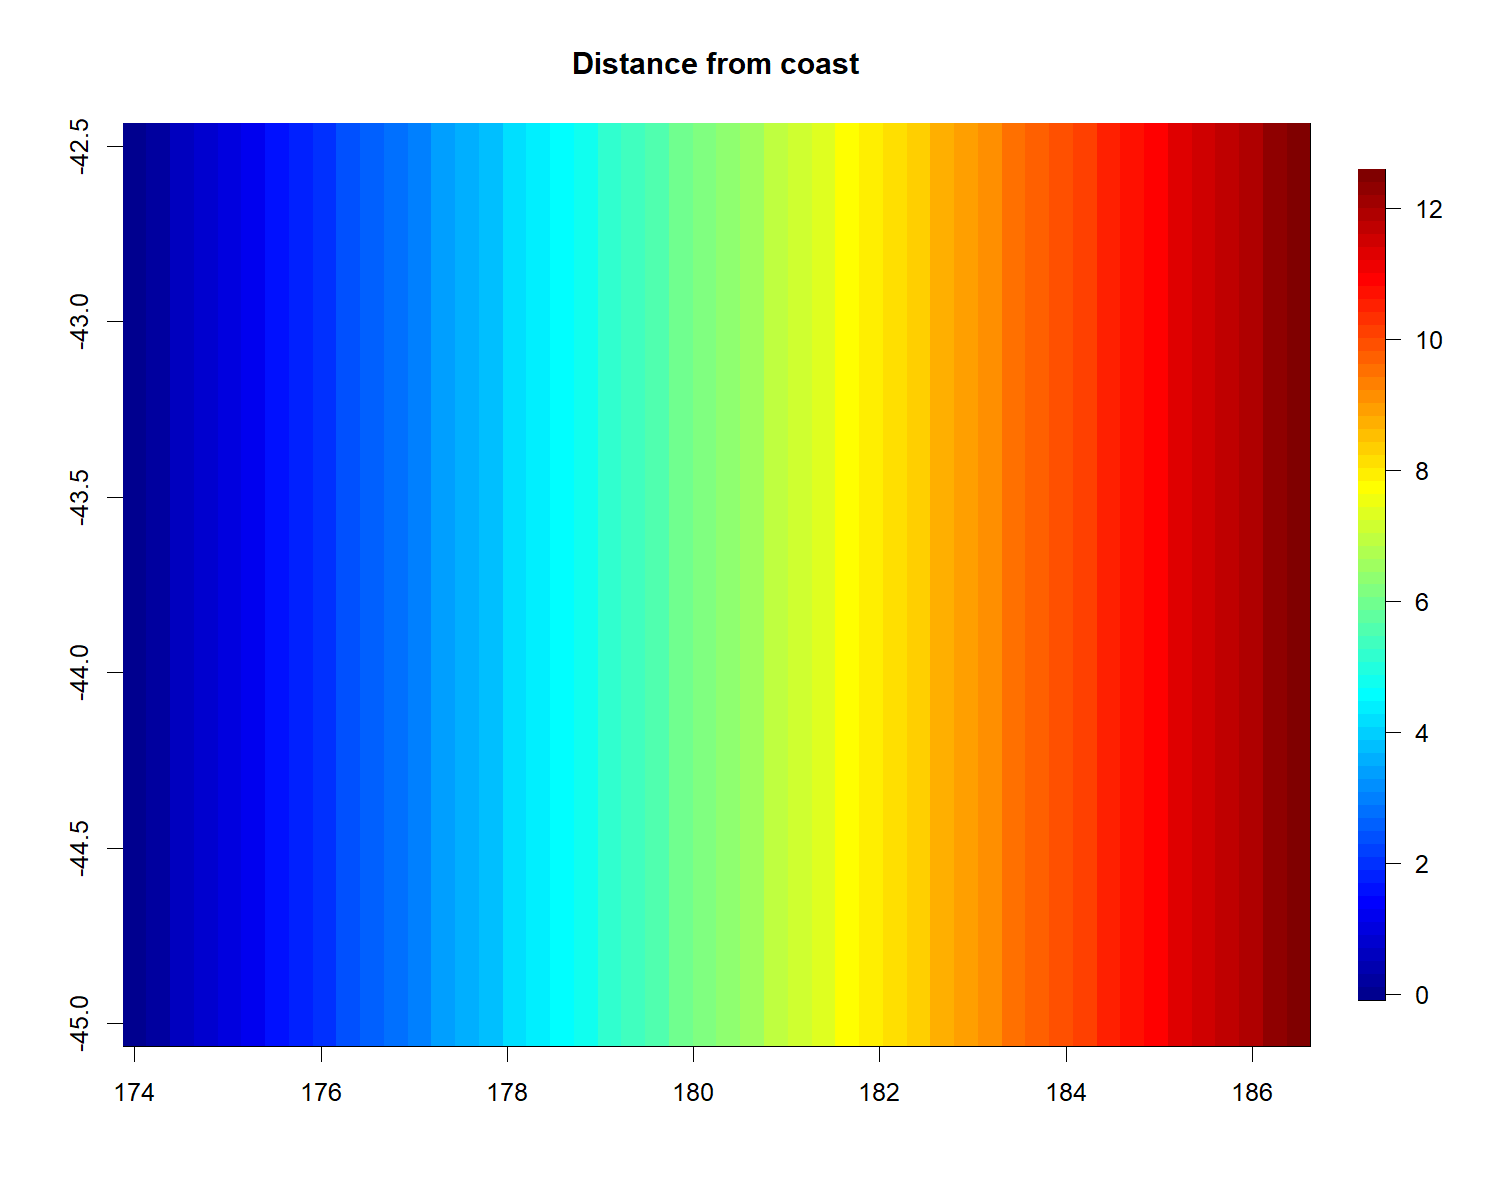
\includegraphics[width=9cm]{Figures/Distance.png} 
	\caption{A layer that represents distance from the eastern coast line}
	\label{fig:distance}%
\end{figure}
Given a numeric layer, you need to assume a preference function (Section~\ref{sec:preference_functions}) which represents the likely areas for effort e.g Figure~\ref{fig:pref_distance}
\begin{figure}[H]
	\centering
	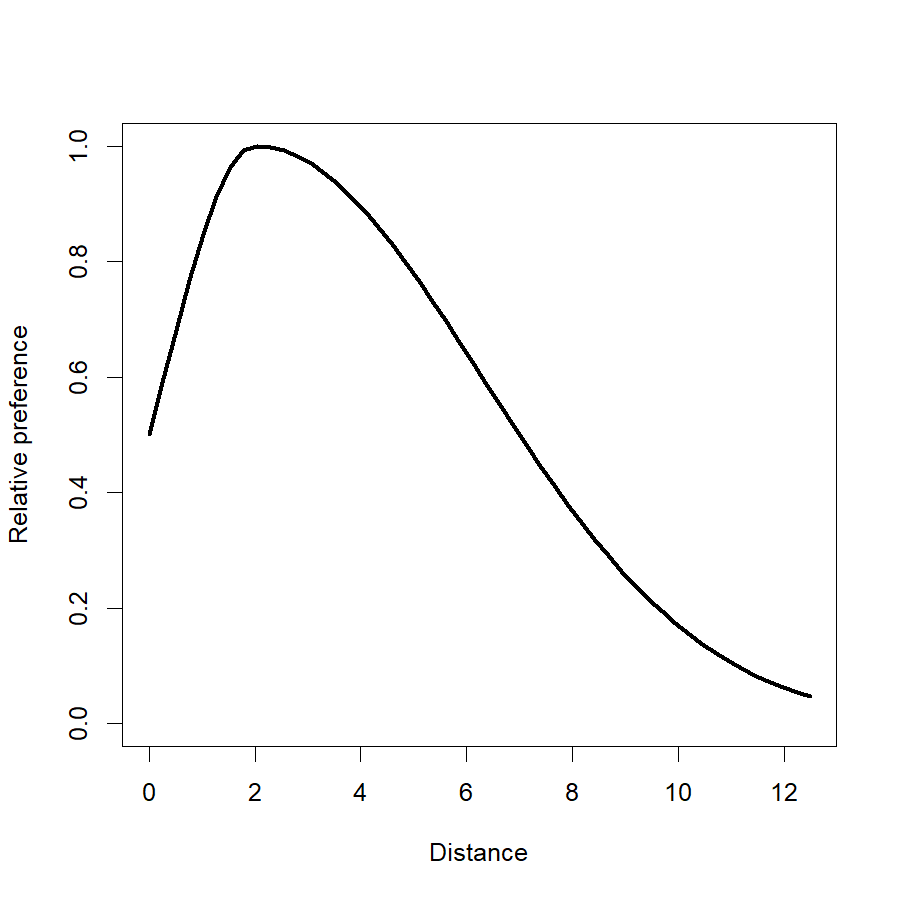
\includegraphics[width=5cm]{Figures/distance_preference_function.png} 
	\caption{Preference function}
	\label{fig:pref_distance}%
\end{figure}
These effort covariates also have an associated weight (multiplier) which is defined by the subcommand \subcommand{preference\_weights}. The resulting relative spatial effort distribution denoted by \(\tilde{E}_{ij}\) is the arithmetic mean of these covariates and the underlying vulnerable biomass.
\begin{equation}
	\tilde{E}_{ij} = \frac{1}{n_k + 1}\sum\limits_{k = 1}^{n_k} P^k_{ij} w_k  \frac{V_{ij}}{\sum_i\sum_j V_{ij}}
\end{equation}
with,
\begin{itemize}
	\item \(V_{ij}\) being vulnerable biomass in cell \(ij\)
	\item \(n_k\) number of covariates
	\item \(P^k_{ij}\) preference value for covariate \(k\)  in cell \(ij\)
	\item \(w_k \) \subcommand{preference\_weights} for covariate \(k\)
	\item \(V_{ij}\) being vulnerable biomass in cell \(ij\)
	\item \(V_{ij}\) being vulnerable biomass in cell \(ij\)
\end{itemize}
%
What this can look like, is take the disatnce from the coast example (Taken from the Example model PreferenceMovementSpatialFishing) if in a given year the vulnerable biomass was distributed as shown Figure~\ref{fig:vulnerable}
\begin{figure}[H]
	\centering
	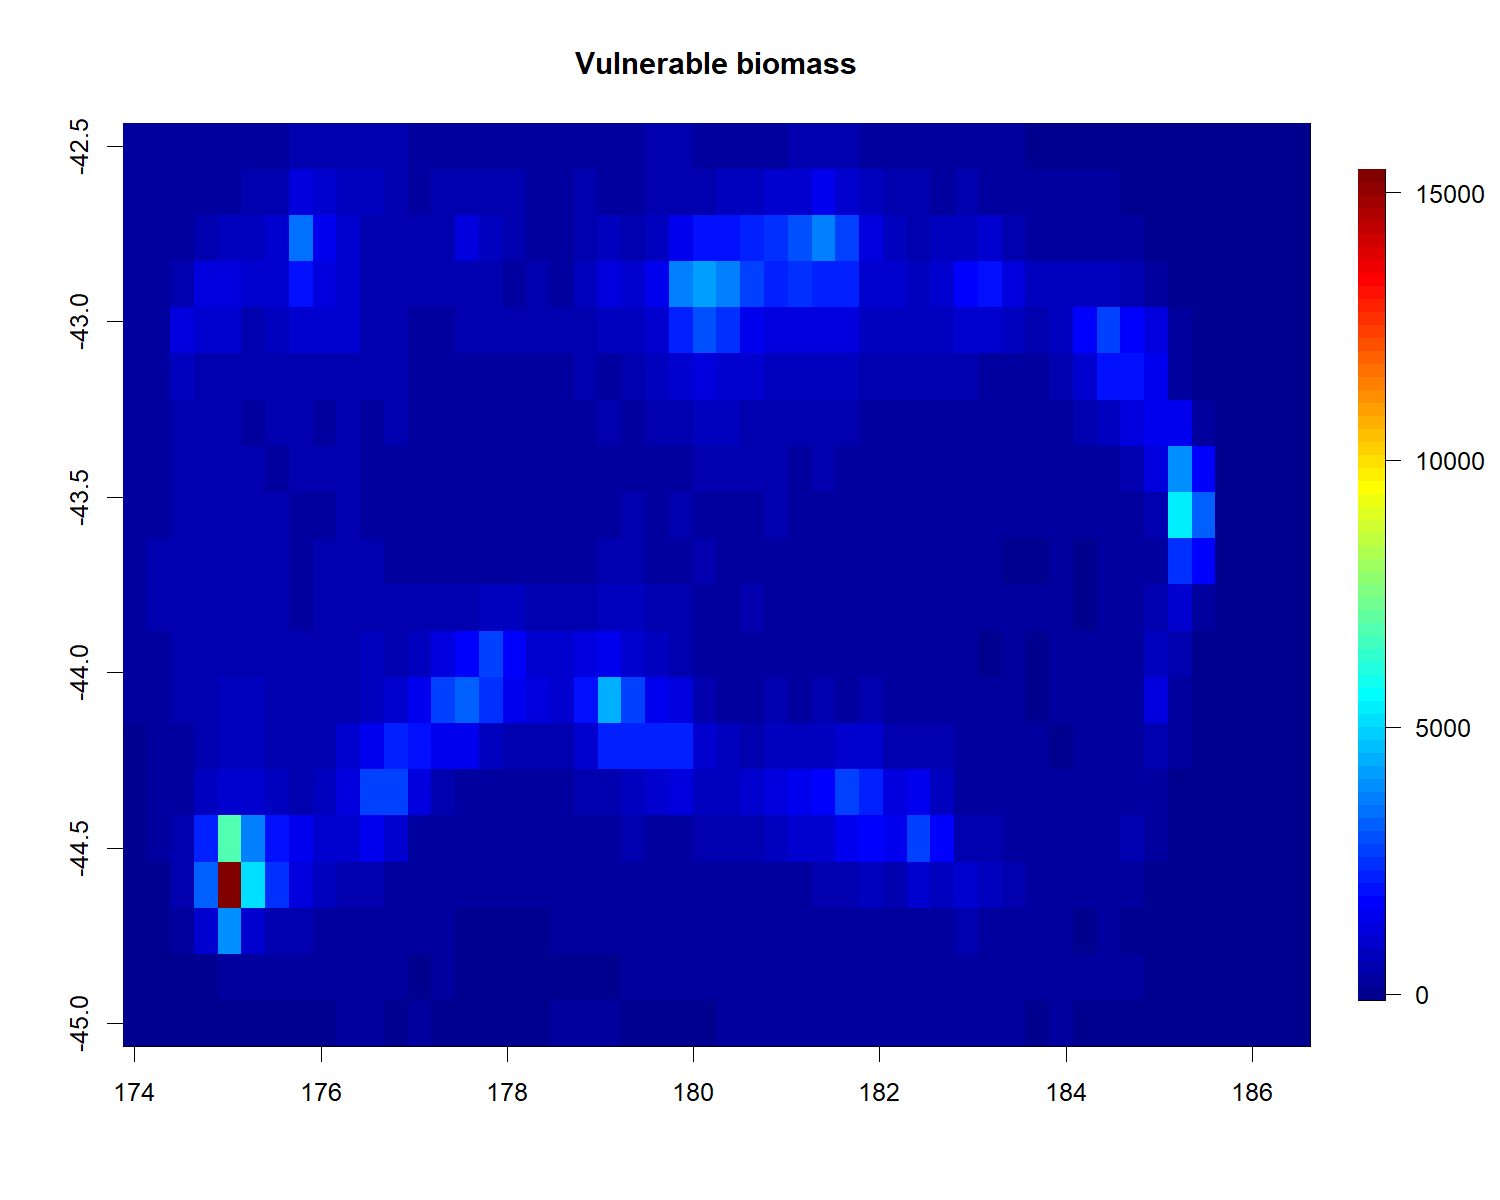
\includegraphics[width=9cm]{Figures/vulnerable_biomass.png} 
	\caption{Vulnerable biomass at the time of fishing}
	\label{fig:vulnerable}%
\end{figure}
%
assuming the \subcommand{preference\_weights} for distance is 0.5 the resulting relative spatial effort distribution (\(\tilde{E}_{ij}\)) would look like Figure~\ref{fig:WIFD}
\begin{figure}[H]
	\centering
	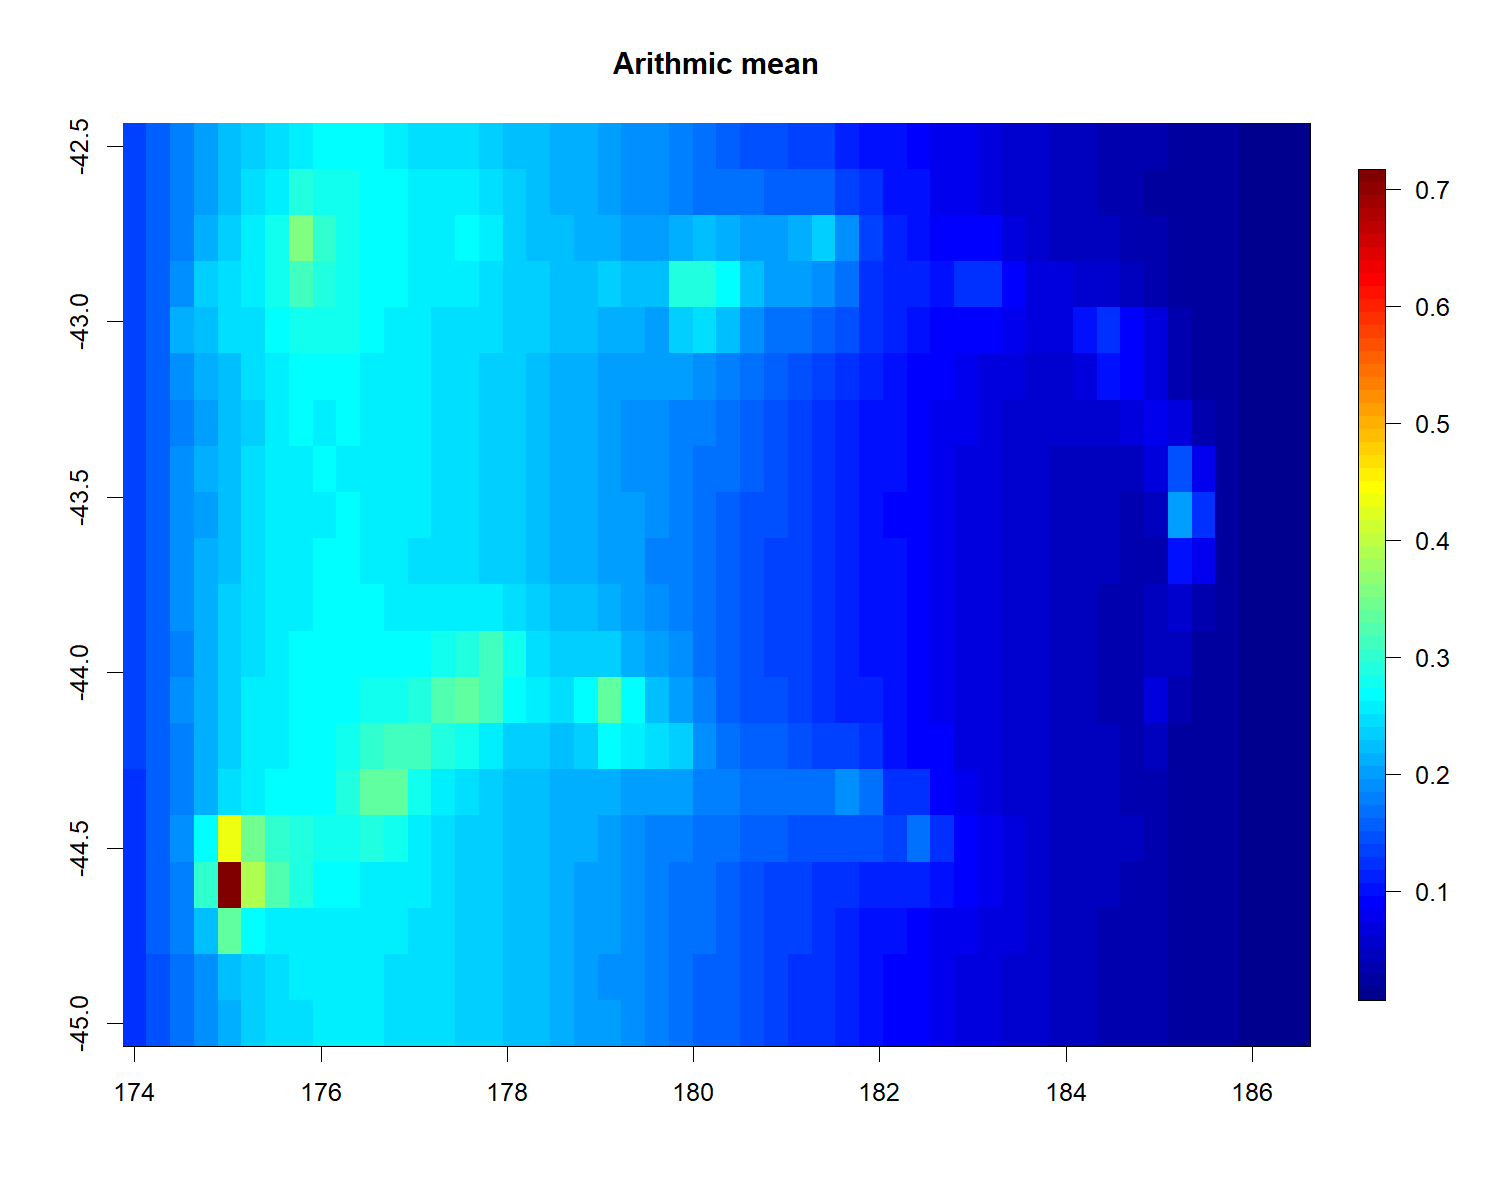
\includegraphics[width=9cm]{Figures/WIFD_arithmic.png} 
	\caption{Vulnerable biomass at the time of fishing}
	\label{fig:WIFD}%
\end{figure}
%
the \subcommand{effort\_values} supplied by the user are then distributed proportional to \(\tilde{E}_{ij}\) as in the previous effort based approach (Section~\ref{para:effort_based_F}). The algorithm then follows exactly the same as Section~\ref{para:effort_based_F}, with the minimisation. To configure this process the following syntax should work.

{\small{\begin{verbatim}
		@process summer_fishery
		type mortality_effort_with_covariates
		years 1991
		catches 2234
		selectivity trawl_selectivity
		minimiser minimiser_for_summer_fishery
		effort_values 0.076 0.089 0.219 0.104 ## for 4 cell model
		preference_functions dist_pref
		preference_layers distance_from_shore
		preference_weights 0.5
		
		@minimiser minimiser_for_summer_fishery
		type numerical_differences
		## play with these if you have trouble minimising or starting value
		iterations	20 
		evaluations 30
		tolerance 0.03
		step_size 0.003
		
		## Preference Functions
		@preference_function dist_pref
		type double_normal
		mu 2
		sigma_l 2
		sigma_r 5
			
		@layer distance_from_shore
		type numeric
		table layer
		0 0.255102 0.5102041 0.7653061
		0 0.255102 0.5102041 0.7653061
		0 0.255102 0.5102041 0.7653061
		0 0.255102 0.5102041 0.7653061
		end_table	
\end{verbatim}}}


\paragraph{Mortality Cull}
Not really a realistic/common mortality event, but useful when looking at movement dynamics. This mortality process will kill all agents in the specified cells.


{\small{\begin{verbatim}
		@process summer_fishery
		type mortality_effort_based
		years 1991
		layer_label kill_all_agents
		
		@layer kill_all_agents
		type integer
		table layer
		0 0 0
		1 1 1 
		end_table
		\end{verbatim}}}
This process will kill all agents in the bottom cells. Any cell with a value > 0, all agents will be removed.
\subsubsection{Movement}\index{Processes!Movement}
\paragraph{Box Transfer}\label{subsubsec:box_transfer}\index{Processes!Movement!Box Transfer}
The box transfer movement process is a simple movement process that is commonly applied in stock assessments. It describes a proportion of individuals moving from a cell to all other cells. This is applied by drawing from a multinomial distribution where an individual will end up. There are two types of movement that users can select for this method; \subcommand{markovian} and \subcommand{natal\_homing}. The difference is with markovian movement the \subcommand{origin\_cell} refers to the cell an individual is currently in, where as if the movement type is natal homing the \subcommand{origin\_cell} refers to the cell that the individual was born in. These are subtle in application but a quite different movement assumptions. A practical note about the two methods natal homing is difficult to thread so may be quite a lot slower (disclaimer I haven't tested it, but I have turned off threading in this process). The probability is not age or length specific and so applies equally to all individuals in a cell. An example of syntax of how you would set this process up for a 3 area model is below.


{\small{\begin{verbatim}
@process Movement
type movement_box_transfer
origin_cell 1-1 2-1 3-1
probability_layers move_from_cell_1 move_from_cell_2 move_from_cell_3
movement_type markovian

@layer move_from_cell_1
type numeric
proportions true
table layer
0.3 0.2 0.5
end_table

@layer move_from_cell_2
type numeric
proportions true
table layer
0.1 0.6 0.3
end_table

@layer move_from_cell_3
type numeric
proportions true
table layer
0.55 0.25 0.2
end_table

\end{verbatim}}}

The above assumes that the probability of movement from one cell to another doesn't change over time. \I{Time varying movement} can be applied by using the numeric meta layers see Section~\ref{sec:layers} for more information. A quick example of how you can apply this following the above example

{\small{\begin{verbatim}
		@layer move_from_cell_1
		type numeric_meta
		years 1990:2000
		layer_labels pre_2000_movement post_2000_movement
		default_layer pre_2000_movement
		
		@layer pre_2000_movement
		type numeric
		proportions true
		table layer
		0.1 0.6 0.3
		end_table
		
		@layer post_2000_movement
		type numeric
		proportions true
		table layer
		0.55 0.25 0.2
		end_table
		\end{verbatim}}}


You can see from the above example that the movement from cell 1 to all other cells has different probabilities from before 2000 and after 2000. The above example could be generalised furthur having a different probability matrix for every year, I kept it simple for illustration.


\paragraph{Preference Based movement}\label{subsubsec:pref_movement}\index{Processes!Movement!Preference Based movement}

The preference in cell $i$ for preference variable $x$ can be described as,
\begin{equation}
P_i^x = f(x_i; \theta)
\end{equation}

where $f(x_i; \theta)$ is a preference function (see Section~\ref{sec:preference_functions}). The overall preference for cell $i$ is the geometric mean of all preference functions from all layers.
\begin{equation}
   P_i = \left(\prod_{n}^{i = 1}P_i^x\right)^{1/n}
\end{equation}
%
where $n$ is the number of preference layers that are involved in the movement process. Once we have the preference for all cells in the spatial domain, we need to calculate the gradient or velocity field in both the $\textbf{X}$ (E-W) and $\textbf{Y}$ (N-S) axis. Currently \IBM\ uses the forward, backwards, and central difference approximation. This obviously sucks as coarse resolution but as we get fine scale models the approximation more accurately will describe the change in preference in each direction. The central approximation has been used in other habitat based preference calculations \citep{phillips2018individual} and is applied like this

\begin{equation}
u_i = \frac{P_{j, i + h} - P_{j, i - h}}{2}
\end{equation}
%
where $h$ is some distance or neighbour cell, this yields us gradient or velocity in both directions then we use a bias random walk to move individuals in space.

\begin{equation}
x_j \sim N(u_i, \sigma_i)
\end{equation}
%
Where $u_i$ is the gradient in the $\textbf{X}$ direction, $D_{i}$ is the diffusion parameter that is scaled based on the habitat preference and $x_j$ is the future location on the X axis of the individual. $D_{i}$ inversely relates to the quality of the preference habitat and a parameter $D_{max}$.

\begin{equation}
D_i = D_{max}\left(1 - \frac{P_i}{\zeta + P_i}\right)
\end{equation}
%
where $\zeta$ is an arbitrary constant controlling the curvature of the function, following \cite{Bertignac1998}.

\begin{equation}
\sigma_i = \sqrt{2 * D_i * t}
\end{equation}
%
Where $t$ is the time steps we have applied the preference movement in annual cycle. This process works well for stationary preference see (FIgure~\ref{fig:static_pref}) The problem with this implementation is that when an individual is in a cell with low preference and no gradient signal, it will randomly jump in any direction (is this biologically sensible?). For example Tuna

\begin{figure}[htp]\label{fig:pref}%
	\centering
	\subfloat[Preference over the spatial domain.]{{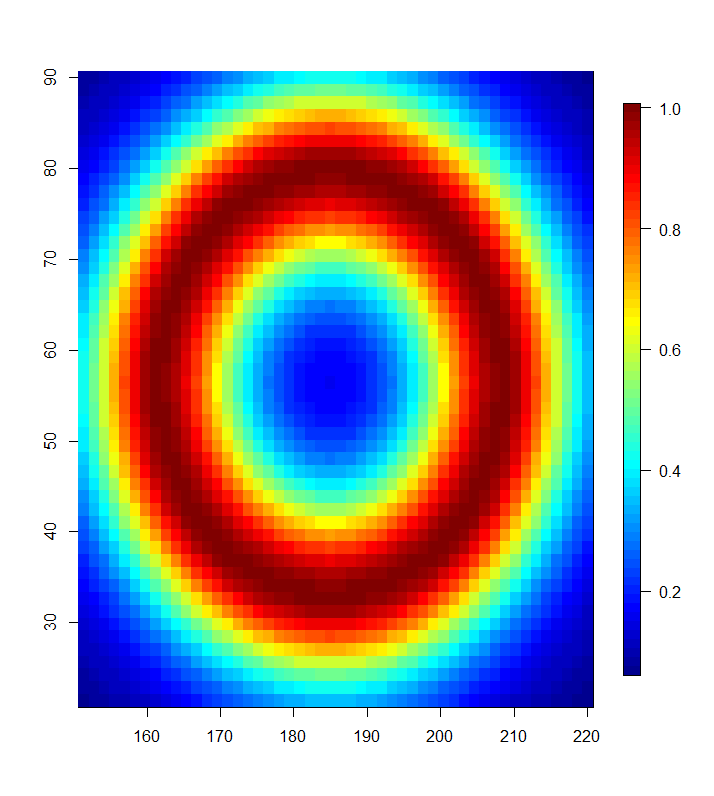
\includegraphics[width=5cm]{Figures/static_preference.png} }}%
	\qquad
	\subfloat[biomass of population with the preference on the left after 30 time steps]{{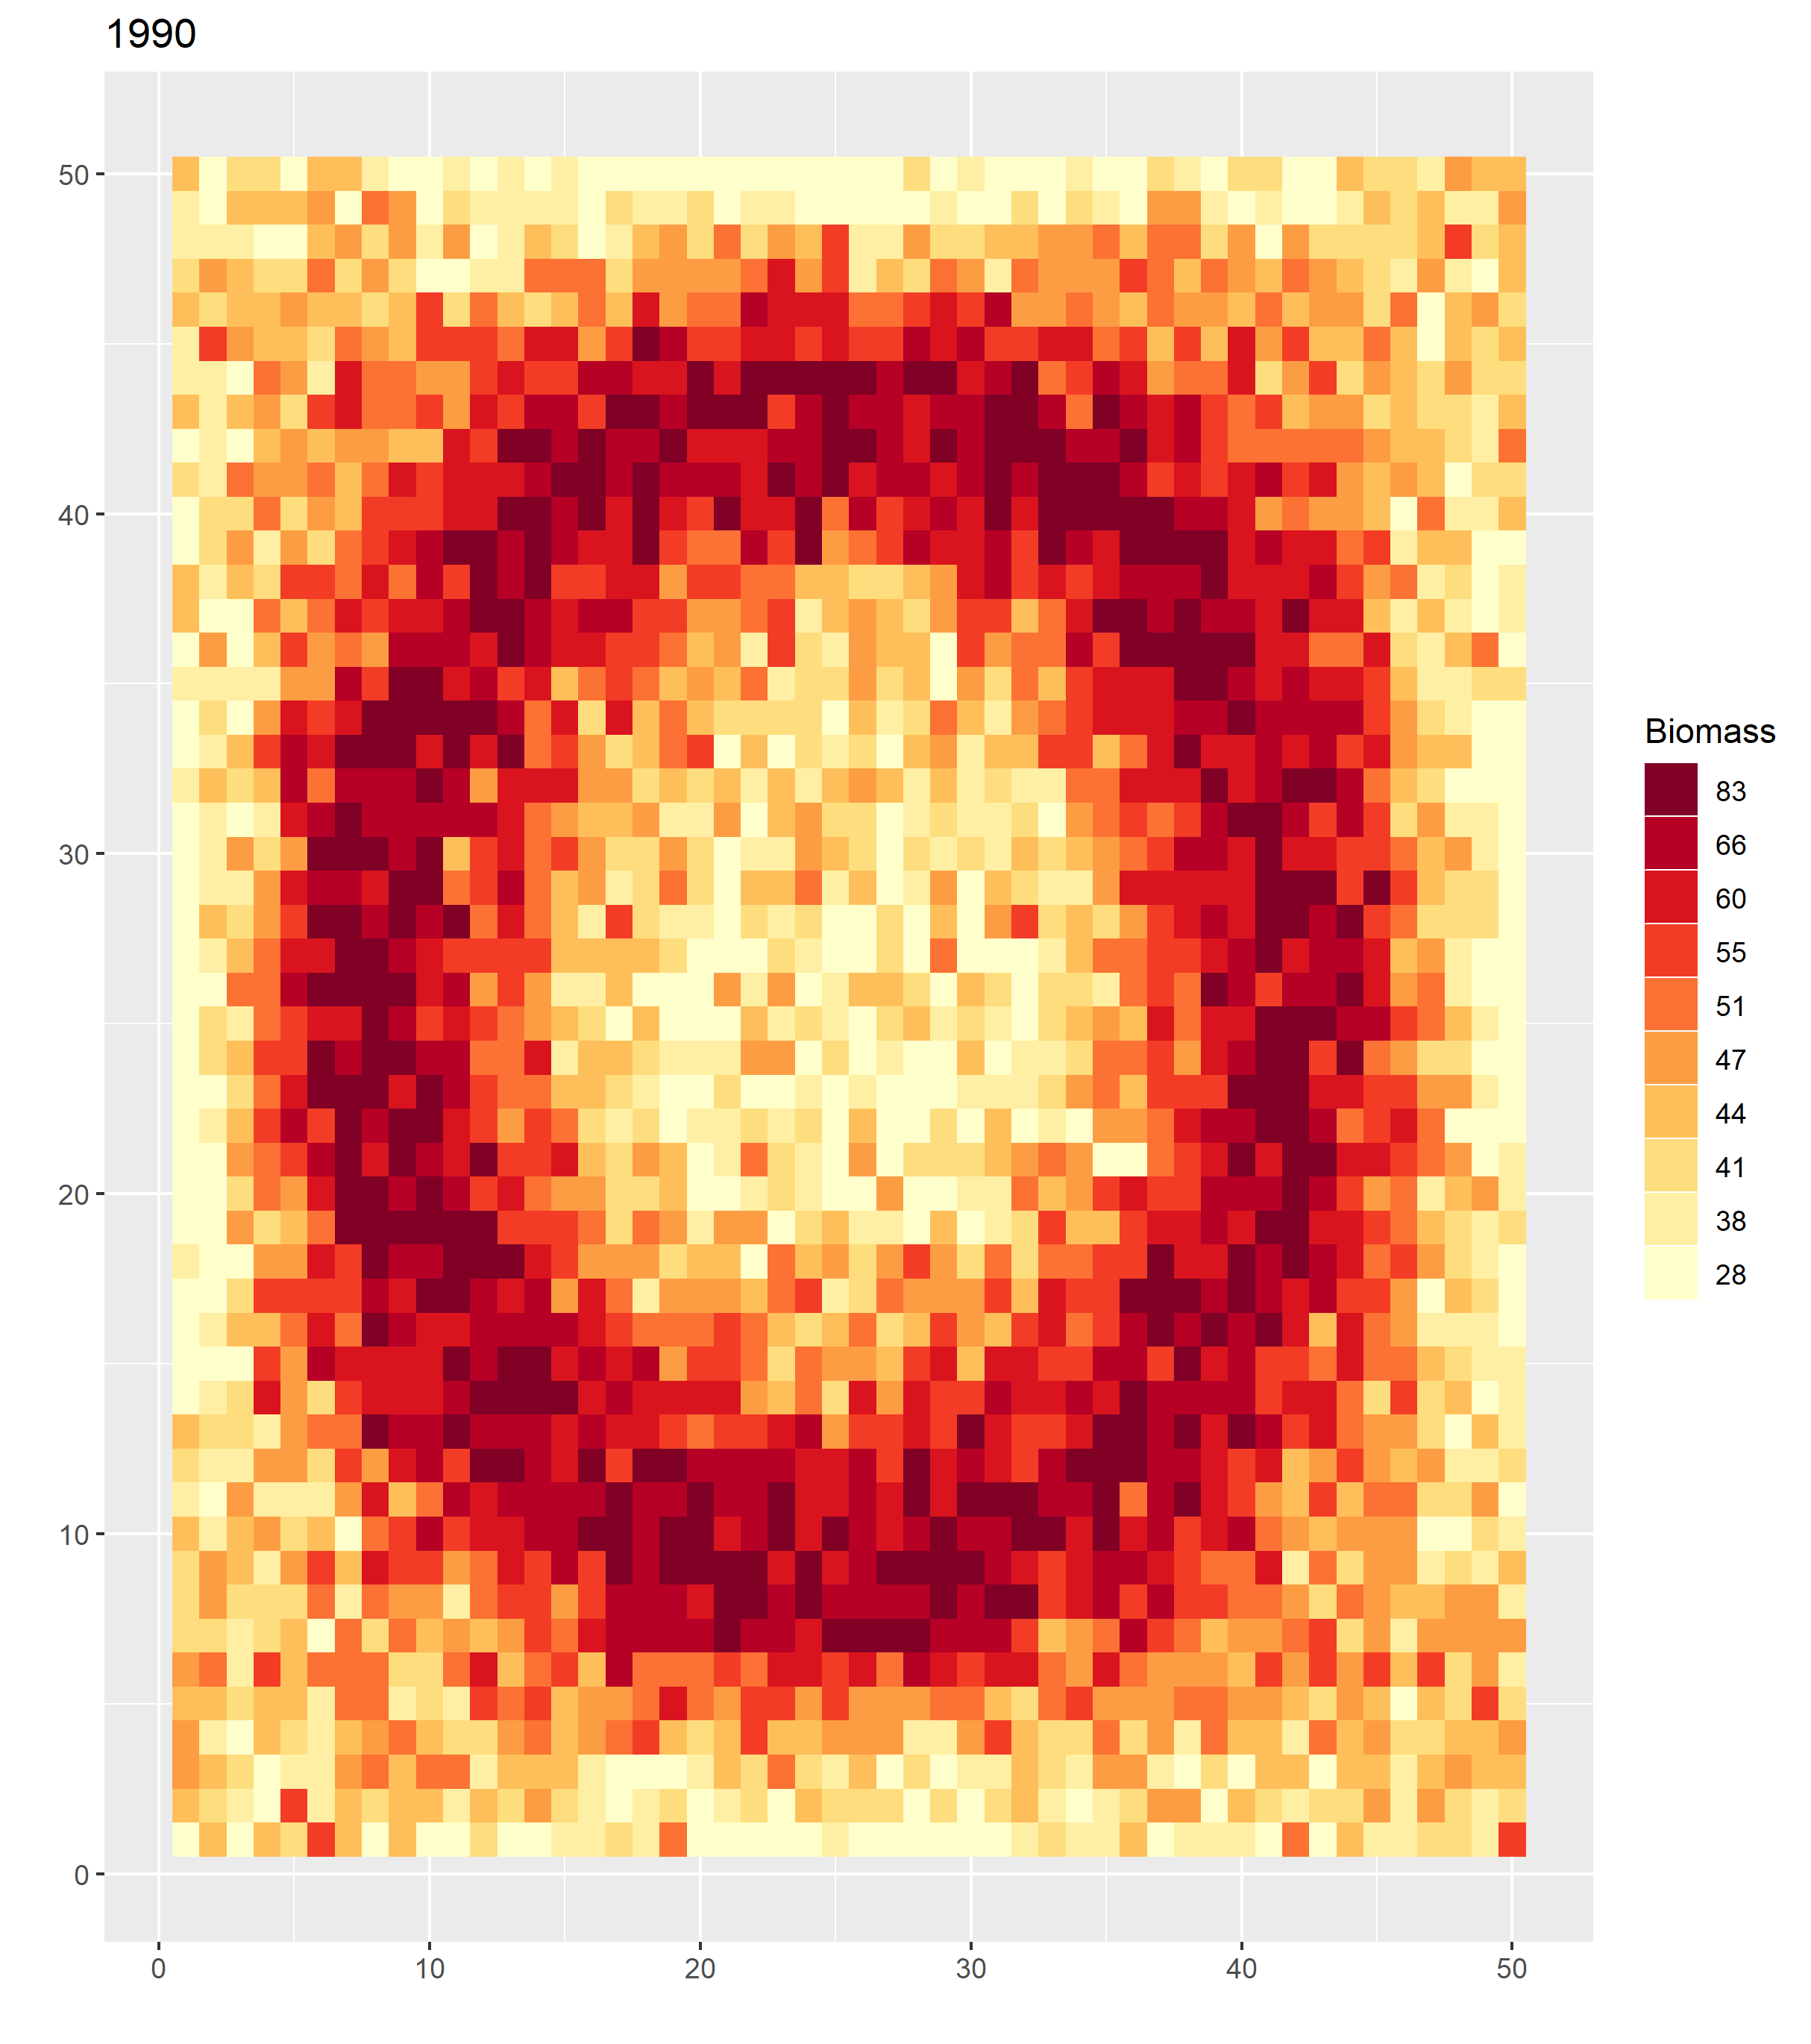
\includegraphics[width=5cm]{Figures/1990_total_biomass_by_cell_move.png} }}%
	\label{fig:static_pref}%
\end{figure}




\subsubsection{Growth}\label{sec:age-at-age}\index{Processes!Growth}
Growth is the process where \IBM\ updates both length and weight for an agent, and the same growth process can be applied over multiple time steps.
\paragraph{Von Bertalanffy with Basic}\label{subsubsec:vonbert_basic}\index{Processes!Growth!Von Bertalanffy with Basic}
This process assumes that weight is an allometric function of length (Equation~\ref{mean_weight}) and that length is an incremental function of time that follows the Von Bertalanffy growth formula. Currently it is also the default growth function used to initialise the equilibrium partition structure. The length from going from one year to the next ($t$ represents a year) follows,

\begin{equation}\label{VB}
\Delta L_{t,i} = p_t((L_{i,\infty} - L_i)(1 - e^{-k_i}))
\end{equation}

\begin{equation}\label{actual_growth}
L_{t+1,i} = L_{t,i} + \Delta L_{t,i}
\end{equation}

If you have multiple time steps in a year and you want growth over all of them, say for example you have monthly time steps and you want to apply $\frac{1}{12}$ of that increment in each year, this can be done by adding the process to all time steps and using the subcommand \subcommand{time\_step\_proportions}. So the growth increment within a time step ($k$) multiplies the annual growth increment by a user defined proportion.

\begin{equation}\label{actual_growth_in_time_step}
L_{t,k + 1,i} = L_{t,k,i} + \Delta L_{t,i}P_k
\end{equation}


Where $i$ indexes each agents own length and growth parameters. If the basic length weight formulation is used, then an agents weight follows the following formula.

\begin{equation}\label{mean_weight}
\bar{w_i} = a_iL_i^{b_i}
\end{equation}

\IBM\ also allow users to seed variability into agent specific growth, two parameters that are allow to vary based on an underlying \textbf{lognormal} distribution are $L_{i,\infty}$ and $k_i$.\\

$$E[L_{i,\infty}] = \text{configuration value}$$

the same goes with $k_i$ and the variability is defined by the $CV$ note that the same cv gets used for randomly drawing both parameters. Aswell as individual variability you can also seed spatial variability in these two parameters. This is done by specifying a layer in the subcommand \subcommand{k\_layer\_label} or \subcommand{linf\_layer\_label}. Then the expectation of the growth parameter assigned to an individual in cell $j,k$ is 

$$E[L_{i,\infty,j,k}] = \text{configuration value}\times \texttt{linf\_layer\_label}_{j,k}$$

So obviously if the layer pointed to by \subcommand{linf\_layer\_label} are all = 1 then the expectation is the same as in the configuration file.\\

When an agent is created (either in initialisation or through a recruitment process) or moves cell, it gets assigned new growth parameters that relate to that cell. This allows for spatial growth, one could hypothesis that environment may explain growth and so different environments over cells will cause different rates of growth. For the growth process you must specify either a spatial layer for mean values of each growth parameter or a single value (if growth doesn't change through space), a distribution and Coefficient of variation (CV). This randomly generates an agent a parameter from that distribution, an example of the syntax in a four area model,

{\small{\begin{verbatim}
		@process von_bert
		type growth_von_bertalanffy_with_basic_weight
		#linf_layer_label L_inf_layer
		linf 101.8
		#k_layer_label k_layer
		k 0.161
		a 2.0e-6 
		b 3.288
		distribution lognormal
		cv 0.15
		time_step_proportions 1 ## if growth occurs in multiple 
		#time step how much growth in each time step
		update_growth_parameters false ## if a individual moves area 
		#do we need to update its growth parameters.
		\end{verbatim}}}
\begin{figure}[h!]\label{fig:age_length}
	\centering
	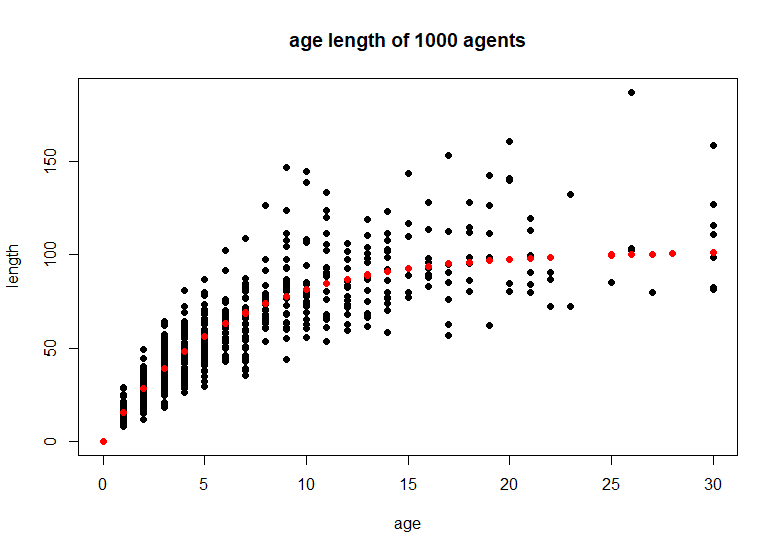
\includegraphics[scale=0.6]{Figures/age-length.png}%
	\caption{An example of the age length relationship from 1000 randomly sampled agents (black dots), red dots signify the assumed deterministic age length relationship.}
\end{figure}


\paragraph{Schnute with Basic}\label{subsubsec:schnute_basic}\index{Processes!Growth!Schnute with Basic}
Following \citep{schnute1981versatile} this applies the generalised Schnute growth increment model following Equation~\ref{eq:schnute}
The distribution relates to the parameters \(\alpha_i\) and \(\beta_i\) for each agent. \(\tau_1\) and \(\tau_2\) are the reference ages with mean length at those reference ages defined as \(y_1\) and \(y_2\) respectively.
\begin{equation}\label{eq:schnute}
	L_{t+1,i} = \bigg(L_{t,i}^{\beta_i} e^{-\alpha_i p_t} + \frac{\left( y_2^{\beta_i} - y_1^{\beta_i} e^{-\alpha_i(\tau_2 - \tau_1) }\right) \left(1 - e^{-\alpha_i p_t}\right)}{\left(1 - e^{-\alpha_i(\tau_2 - \tau_1)}\right)}\bigg)^{1/\beta_i}
\end{equation}

{\small{\begin{verbatim}
# Growth
@process Growth
type growth_schnute_with_basic_weight
y1 24.5
y2 104.8
tau1 1 
tau2 20 
alpha 0.131
beta 1.70
t0 24.5
a 2.0e-9
b 3.288
cv 0.15
update_growth_parameters false ## if an agent moves we don't update growth info
distribution lognormal
time_step_proportions 1.0
\end{verbatim}}}



\subsubsection{Tagging}\index{Processes!Tagging}\label{subsub:tag}
Tagging is a process where by agents get tagged and is a tag release event. This is a simple process where a user defines a selectivity that describes the probability of being captured for tagging, and also a number of tags that are released in each spatial cell. I have usually applied tagging before a mortality process which is where tag recaptures occur (Section~\ref{sec:mortality}). Also you will need to specify mortality processes to scan for tagged fish if you want any information on recapture probabilities. This will be printed in the process information.

{\small{\begin{verbatim}
@process Tagging_event
type tagging
years 1990
selectivities Sel_LL
tag_release_layer tag_1990
handling_mortality 0.12

@layer tag_1990
type integer
table layer
12314
9854
4686
end_table
\end{verbatim}}}

The algorithm for this process follows
\begin{enumerate}
	\item randomly select an agent with replacement if it is not already tagged ($U() \leq S_a$)
	\item assign tag, and meta information, when it was tagged, where it was tagged etc.
	\item if the agent represents multiple individuals strip it out and assign its scalar $s_i = 1$
	\item See if it died from handling mortality if ($U() \leq H$) where $H$ is the subcommand \subcommand{handling\_mortality}
\end{enumerate}

\subsection{\I{Derived Quantities}\label{sec:derived-quantities}}
Derived quantities surround a mortality block and so the value of the derived quantity is calculated twice, once before the mortality block (Pre-Execute), and once after (Execute). The final value is an interpolation based on how much mortality the user wants to take into account when calculating derived quantities. If users set the \subcommand{proportion\_through\_mortality\_block} parameter equal to one or zero then only one calculation is taken, and can reduce the run time of some models, so it is worth exploring.

\begin{equation}
	B_p = (1 - p)B + pB'
\end{equation}
where $B_p$ is the interpolated derived quantity after $p$ proportion through the mortality block, $B$ is the quantity at the beginning of the mortality block and $B'$ is the derived quantity at the end of the mortality block.\\

Derived quantities can be used either to report the state of a particular components of the population, or used in populations. For example in the Beverton Holt recruitment process (Section~\ref{subsubsec:bev-holt-recruitment}) users must define a subcommand \subcommand{ssb} which is a derived quantity. So this can be a useful tool to incorporate density dependence based processes.

\paragraph*{Biomass}\label{para:biomass}
Users must specify cells in which to calculate the derived quantity over using the subcommand \subcommand{biomass\_layer\_label}
\begin{equation}
	B = \sum_i \text{if }(U() \leq S_a)\text{I } \bar{w_i} \times s_i
\end{equation}
where for an age based selectivity where $S_a$ is the probability of being included in this derived quantity, if the summary is age based, I is a 0 or 1 depending on the condition of the if statement, $\bar{w_i}$ is the weight of the agent and $s_i$ is the scalar of the agent i.e. how many individuals that agent represents.
{\small{\begin{verbatim}
	@derived_quantity Total_biomass_in_Summer
	type biomass
	biomass_layer_label Base
	selectivity All
	time_step Summer
	proportion_through_mortality_block 0.0
	
	@selectivity All
	type constant
	c 1
\end{verbatim}}}


\paragraph*{Mature Biomass}\label{para:mature_biomass}

\begin{equation}
B = \sum_i if(mature = 1)\text{ I } \bar{w_i} \times s_i
\end{equation}
where $s_i$ is the scalar of the agent i.e. how many individuals that agent represents.

{\small{\begin{verbatim}
		@derived_quantity SSB
		type mature_biomass
		biomass_layer_label SSB_layer
		time_step time_step_one
		proportion_through_mortality_block 0.0
\end{verbatim}}}
	
\paragraph*{Abundance}\label{para:abundance}

\begin{equation}
B = \sum_i \text{if }(U() \leq S_a)\text{I } s_i
\end{equation}
where for an age based selectivity where $S_a$ is the probability of being included in this derived quantity, if the summary is age based, I is a 0 or 1 depending on the condition of the if statement,$s_i$ is the scalar of the agent i.e. how many individuals that agent represents.
{\small{\begin{verbatim}
		@derived_quantity Total_abundance_in_Summer
		type abundance
		layer_label Base
		selectivity All
		time_step Summer
		proportion_through_mortality_block 0.0
		
		@selectivity All
		type constant
		c 1
\end{verbatim}}}


\subsection{\I{Selectivities}\label{sec:selectivities}}
A selectivity is a function that can have a different value for each age class or length bin. Selectivities are used throughout \IBM\ to interpret observations or to modify the effects of processes on each age class or length bins (Section \ref{sec:population-section}). \IBM\ implements a number of different parametric forms, including logistic, knife edge, and double normal selectivities. Selectivities are defined in there own command block (\command{selectivity}), where the unique label is used by observations or processes to identify which selectivity to apply.

Selectivities are indexed by age, with indices from \argument{min\_age} to \argument{max\_age}. For example, for a logistic age-based selectivity with $50\%$ selected at age $5$ and $95\%$ selected at age $7$, would be defined by the \subcommand{type}=\argument{logistic} with parameters $a_{50}=5$ and $a_{to95}=(7-5)=2$. The value of the selectivity at age $x=7$ is $0.95$, and the value at age $x=3$ is $0.05$. Note, while selectivities can be length based, use with caution as more testing is needed for this functionality.

The function values for some choices of parameters, for some selectivities, can result in a computer numeric overflow error (i.e., the number calculated from parameter values is either too large or too small to be represented in computer memory). \IBM\ implements range checks on some parameters to test for a possible numeric overflow error before attempting to calculate function values. For example, the logistic selectivity is implemented such that if $(a_{50}-x)/a_{to95} > 5$ then the value of the selectivity at $x=0$, i.e., for $a_{50}=5$, $a_{to95}=0.1$, then the value of the selectivity at $x=1$, without range checking would be $7.1 \times 10^{-52}$. With range checking, that value is $0$ (as $(a_{50}-x)/a_{to95}=40 > 5$).

The available selectivities are;

\begin{itemize}
  \item Constant
  \item Knife-edge
  \item All values
  \item All values bounded
  \item Increasing
  \item Logistic
  \item Inverse logistic
  \item Logistic producing
  \item Double normal
  \item Double exponential
% \item Cubic spline (Not yet implemented)
\end{itemize}

The available selectivities are described below.

\subsubsection[Constant]{{constant}}

\begin{equation}
f(x)=C
\end{equation}

The constant selectivity has the parameter C. 

\subsubsection[Knife-edge]{\argument{knife\_edge}}
\begin{equation}
f(x)= \begin{cases}
  0, & \text{if $x < E$} \\
  \alpha, & \text{if $x \ge E$}\\ 
  \end{cases} 
\end{equation}

The knife-edge ogive has the estimable parameter E and a scaling parameter $\alpha$, where the default value of $\alpha = 1$.

\subsubsection[All-values]{\argument{all\_values}}\index{Selectivities!All-values}

\begin{equation}
f(x)=V_x
\end{equation}

The all-values selectivity has parameters $V_{low}$, $V_{low+1}$ \ldots $V_{high}$. Here, you need to provide the selectivity value for each age class.

\subsubsection[All-values-bounded]{\argument{all\_values\_bounded}}\index{Selectivities!All-values-bounded}

\begin{equation}
f(x)=\begin{cases}
		 0, & \text{if $x < L$} \\
		 V_x, & \text{if $L \le x \le H$} \\
		 V_H, & \text{if $x > H$}
  \end{cases}
\end{equation}

The all-values-bounded selectivity has parameters  $L$, $H$, $V_L$, $V_{L+1}$ \ldots $V_H$. Here, you need to provide an selectivity value for each age class from $L \ldots H$.

\subsubsection[Increasing]{\argument{increasing}}\index{Selectivities!Increasing}

\begin{equation} 
f(x)=\begin{cases}
	  0, & \text{if $x < L$} \\
	  f(x-1)+ \pi_x(\alpha-f(x-1)), & \text{if $L \le x \le H$} \\
	  f(\alpha), & \text{if $x \ge H$} \\  
  \end{cases}
\end{equation}

The increasing ogive has parameters $L$ and $H$, $\pi_L$, $\pi_{L+1}$ \ldots $\pi_H$ (but if these are estimated, they should always be constrained to be between 0 and 1). $\alpha$ is a scaling parameter, with default value of $\alpha = 1$. Note that the increasing ogive is similar to the all-values-bounded ogive, but is constrained to be non-decreasing.

\subsubsection[Logistic]{\argument{logistic}}\index{Selectivities!Logistic}

\begin{equation}
  f(x) = \alpha / [1+19^{(a_{50}-x)/a_{to95}}]
\end{equation}
 
The logistic selectivity has parameters $a_{50}$ and $a_{to95}$. $\alpha$ is a scaling parameter, with default value of $\alpha = 1$. The logistic selectivity takes values $0.5 \alpha$ at $x=a_{50}$ and $0.95 \alpha$ at $x=a_{50}+a_{to95}$. 

\subsubsection[Inverse logistic]{\argument{inverse\_logistic}}\index{Selectivities!Inverse-logistic}

\begin{equation}
  f(x) = \alpha - \alpha / [1+19^{(a_{50}-x)/a_{to95}}]
\end{equation}
 
The inverse logistic selectivity has parameters $a_{50}$ and $a_{to95}$. $\alpha$ is a scaling parameter, with default value of $\alpha = 1$. The logistic selectivity takes values $0.5 \alpha$ at $x=a_{50}$ and $0.95 \alpha$ at $x=a_{50}-a_{to95}$. 

\subsubsection[Logistic producing]{\argument{logistic\_producing}}\index{Selectivities!Logistic-producing}

\begin{equation} 
f(x)=\begin{cases}
	  0, & \text{if $x < L$} \\
	  \lambda(L), & \text{if $x=L$} \\
	  \left( \lambda(x)-\lambda(x-1) \right) / \left( 1-\lambda(x-1) \right), & \text{if $L < x < H$} \\
	  1, & \text{if $x \ge H$} \\  
  \end{cases}
\end{equation}

The logistic-producing selectivity has the parameters $L$ and $H$, $a_{50}$ and $a_{to95}$. $\alpha$ is a scaling parameter, with default value of $\alpha = 1$. For category transitions, $f(x)$ represents the proportion moving, not the proportion that have moved. This selectivity was designed for use in an age-based model to model maturity. In such a model, a logistic-producing maturation selectivity will (in the absence of other influences) make the proportions mature follow a logistic curve with parameters $a_{50}$, $a_{to95}$.

\subsubsection[Double-normal]{\argument{double\_normal}}\index{Selectivities!Double-normal}

\begin{equation}
  f(x) = \begin{cases}
    \alpha 2^{-[(x- \mu)/\sigma_L ]^2}, & \text{if $x \leq \mu$} \\
    \alpha 2^{-[(x- \mu)/\sigma_R ]^2}, & \text{if $x \ge \mu$}\\
  \end{cases}
\end{equation} 

The double-normal selectivity has parameters $\mu$, $\sigma_L$, and $\sigma_R$. $\alpha$ is a scaling parameter, with default value of $\alpha = 1$. It has values $\alpha$ at $x=\mu$

\subsubsection[Double-exponential]{\argument{double\_exponential}}\index{Selectivities!Double-exponential}

\begin{equation} 
f(x)=\begin{cases}
	  \alpha y_0(y_1 / y_0)^{(x-x_0)/(x_1-x_0)}, & \text{if $x \le x_0$} \\
	  \alpha y_0(y_2 / y_0)^{(x-x_0)/(x_2-x_0)}, & \text{if $x > x_0$} \\
  \end{cases}
\end{equation}

The double-exponential selectivity has  parameters $x_1$, $x_2$, $x_0$, $y_0$, $y_1$, and $y_2$.  $\alpha$ is a scaling parameter, with default value of $\alpha = 1$. It can be `U-shaped'. Bounds for $x_0$ must be such that $x_1 < x_0 < x_2$. With $\alpha=1$, the selectivity passes through the points $(x_1, y)$, $(x_0, y_0)$, and $(x_2, y_2)$. If both $y_1$ and $y_2$ are greater than $y_0$ the selectivity is `U-shaped' with minimum at $(x_0, y_0)$.


Selectivities \subcommand{all\_values} and \subcommand{all\_values\_bounded} can be addressed in additional priors using the following syntax,

{\small{\begin{verbatim}
		@selectivity maturity
		type all_values
		v 0.001 0.1 0.2 0.3 0.4 0.3 0.2 0.1
		
		## encourage ages 3-8 to be smooth.
		@additional_prior smooth_maturity
		type vector_smooth
		parameter selectivity[maturity].values{3:8}
		
		\end{verbatim}}}
	
\subsection{\I{Preference Functions}\label{sec:preference_functions}}
Preference functions are a class of equations that describe the preference for of agents to a covariate used to describe movement in the preference based movement process (Section~\ref{subsubsec:pref_movement}). Currently there are only three options

\begin{enumerate}
	\item Double normal
	\item Logistic
	\item Normal
\end{enumerate}

These are the same equations as in the selectivities (Section~\ref{sec:selectivities}), but that instead of specifying the vulnerability for age or length they describe the preference for a user defined covariate or explanatory variable so the units are completely user defined.
\subsubsection[Double-normal]{\argument{double\_normal}}\index{Preference Functions!Double-normal}

\begin{equation}
f(x) = \begin{cases}
\alpha 2^{-[(x- \mu)/\sigma_L ]^2}, & \text{if $x \leq \mu$} \\
\alpha 2^{-[(x- \mu)/\sigma_R ]^2}, & \text{if $x \ge \mu$}\\
\end{cases}
\end{equation} 

The double-normal preference function has parameters $\mu$, $\sigma_L$, and $\sigma_R$. $\alpha$ is a scaling parameter, with default value of $\alpha = 1$. It has values $\alpha$ at $x=\mu$.

\subsubsection[Logistic]{\argument{logistic}}\index{Preference Functions!Logistic}

\begin{equation}
f(x) = \alpha / [1+19^{(a_{50}-x)/a_{to95}}]
\end{equation}

The logistic preference function has parameters $a_{50}$ and $a_{to95}$. $\alpha$ is a scaling parameter, with default value of $\alpha = 1$. The logistic selectivity takes values $0.5 \alpha$ at $x=a_{50}$ and $0.95 \alpha$ at $x=a_{50}+a_{to95}$. 

\subsubsection[Normal]{\argument{double\_normal}}\index{Preference Functions!Normal}

\begin{equation}
f(x) = 
\alpha 2^{-[(x- \mu)/\sigma]^2}
\end{equation} 

The normal preference function has parameters  $\sigma$, and $\mu$. $\alpha$ is a scaling parameter, with default value of $\alpha = 1$. It has values $\alpha$.

\subsection{\I{Time Varying Parameters}\label{sec:time_var}}

\IBM\ has the functionality to vary some parameters annually between the start and final year of a model run. This can be for blocks of years or specific years. For years that are not specified the parameter will default to the input. Method types for time varying a parameter are; \subcommand{constant}, \subcommand{random\_walk}, \subcommand{exogenous}, \subcommand{linear}, \subcommand{annual\_shift}, \subcommand{random\_draw}. This allows users to let a parameter be known in a year, be the result of a deterministic equation, or stochastic. 

When allowing removals to have annual varying, selectivities and other more realistic model components, simulated observations more closely model real data and associated conclusions become more useful. Another driver for implementing time-varying parameters was allowing mean or location parameters of selectivities to change between years based on an explanatory variable. An example of this is in the New Zealand Hoki fishery where we allow the $\mu$ and $a_{50}$ parameters to shift depending on when the fishing season occurs. Descriptive analysis showed that when fishing was earlier relative to other years smaller fish were caught and vice versa.

\subsubsection[Constant]{\argument{constant}}\index{Time Varying Parameters!Constant}
Allows a parameter to have an alternative value during certain years, which can be estimated.
{\small{\begin{verbatim}
		@time_varying m_time_var
		type constant
		parameter process[natural_mortality].m
		years 1975:1988
		values 0.123
		\end{verbatim}}}


\subsubsection[Random Walk]{\argument{random\_walk}}\index{Time Varying Parameters!Random Walk}

A random deviate is added into the last value drawn from a standard normal distribution. This has an estimable parameter $\sigma_p$ for each time varying parameter $p$. For reproducible modelling, it is highly recommended that users set the seed (see Section~\ref{sec:command-line-arguments}) when using stochastic functionality like this, otherwise reproducing models becomes almost impossible.
{\small{\begin{verbatim}
		@time_varying m_time_var
		type random_walk
		parameter process[natural_mortality].m
		distribution normal
		mean 0.123
		sigma 0.05
		\end{verbatim}}}

A constraint whilst using this functionality is that a parameter cannot be less than 0.0, if it is \IBM\ sets it equal to 0.01.

\subsubsection[Annual shift]{\argument{annual\_shift}}\index{Time Varying Parameters!Annual shift}

A parameter generated in year $y$ ($\theta'_y$) depends on the value specified by the user ($\theta_y$) along with three coefficients $a,b$ and $c$ as follows,

\begin{equation}
\bar{\theta}_y = \frac{\sum_{y}^Y\theta_y}{Y}
\end{equation}

\begin{equation}
\theta'_y = a \bar{\theta}_y + b\bar{\theta}_y^{2} + c\bar{\theta}_y^{3}
\end{equation}

\subsubsection[Exogenous]{\argument{exogenous}}\index{Time Varying Parameters!Exogenous}

Parameters are shifted based on an exogenous variable, an example of this is an exploitation selectivity parameters that may vary between years based on known changes in exploitation behaviour such as season, start time, and average depth of exploitation.

\begin{equation}
\delta_y = a(E_y - \bar{E})
\end{equation}

\begin{equation}
\theta'_y = \theta_y + \delta_y
\end{equation}

where $\delta_y$ is the shift or deviation in parameter $\theta_y$ in year $y$ to generate the new parameter value in year $y$ ($\theta'_y$). $a$ is an estimable shift parameter, $E$ is the exogenous variable and $E_y$ is the value of this variable in year $y$. For more information readers can see \cite{francis_03}.


\subsection{\I{Tips setting up configuration files}\label{sec:tips}}
\IBM\ can take a while if you have a complex spatial model and complex life history. So there are some tips and tricks that I have come found can be useful when setting up configuration files.

\subsubsection*{Debugging a model}
When initially setting up a model set initialisation years low and number of agents low, because there is a lot going on in this model it is best to get up and run (which is a good feeling). Also I would advice setting up the population and report components, only once you are happy with that that I would suggest bringing in Observations. Advice I always struggle to keep to is, start very basic and build complexity, otherwise say good bye to time and hello to frustration. Once you are happy with your model then I would suggest increase initialisation years and number of agents.

\subsubsection*{The initialisation Phase}
The first thing you wont to nail down before getting gun hoe on the configuration and complex dynamics you want to get a model that reaches an appropriate initialisation state \emph{quickly!}. So my suggestion is to not worry about fishing in the first instance, set the \subcommand{start\_year} and \subcommand{final\_year} one year apart and play with the initialisation phase commands to see how to efficiently reach a desired initial state. The parameters I am talking about are the subcommands \subcommand{years} and \subcommand{layer\_label}. The \subcommand{years} parameter sets how many annual cycles to run through to set your initialisation state, you want this as small as possible. So my advice is run the model with a range of \subcommand{years} say 5, 10, 20, 30, 40, 50 and 100 to find out how sensitive your initial state is to this. You find that you have to make a compromise between speed and accuracy, unfortunately life is full of such compromises. To see some example \R\ code on how I compare initialisation see Section~\ref{sec:post-processing}.

Along with the \subcommand{years} parameter you can also set the spatial distribution of the initial seeding of agents through the \subcommand{layer\_label}, if you have a spatial model with movement this would be an interesting one to play with. So pretty much my advice is tweak these initialisation parameters as much as you can before you move onto fishing and generate observations, it will be well worth your while if you treasure time.

\subsubsection*{The number of agents in the system} 
This one should be obvious and we suggest that you play with the initialisation parameter \subcommand{number\_of\_agents} to see how sensitive model outputs are to this parameter. The less agents in the system the faster your model will run, however the less agents the more coarse you model becomes because then an entity all of a sudden represents 1000 if not 10000 entities, so once again we return to a compromise.

\subsubsection*{The number of threads available}
\textbf{Disabled} was not implemented correctly the first time, still to many shared resources.. 
%\IBM\ is threaded using the OpenMP C++ library, by default \IBM\ will set the number threads available equal to number available on your machine minus 1. You can set this through the \command{model} parameter \subcommand{max\_threads\_to\_use}, we suggest you set this to the number of spatial cells in the system, there might be more overheads with making more threads available than the model will ever use (disclaimer I haven't tested this). 

\subsubsection*{more ways than one to skin a cat} 
Hopefully throughout the process and derived quantities I have discussed alternative ways to set up a similar model. Given there generality of the program there are more than one way to approximate dynamics and some will be more computationally quicker than others. So have a play around but try and keep the number of times we iterate over the state as small as possible, as you will get significant time saving. It is also possible to make your own specific process that does a range of processes at one time, thus saving a lot of time. This can be easily done by looking over the current processes and taking the functionality that has been tested and copy them in to a new file.
